% !TeX program = pdflatex
\documentclass[11pt, letterpaper,oneside]{memoir}
\usepackage[margin=1in]{geometry}
\usepackage[utf8]{inputenc}
\usepackage[USenglish]{babel}
%\usepackage[english]{fancyref}  
\usepackage{graphicx}
\usepackage{tabularx}
\usepackage{booktabs}
\usepackage{pdfpages}
\usepackage{float}
\usepackage{stix}
\usepackage{url}
\usepackage{eso-pic}
\usepackage{hyperref}
\usepackage{footnotebackref}
\usepackage[inline]{enumitem}
\usepackage{amsmath}
\usepackage{amssymb}
\usepackage{amsthm}
\usepackage{commath}
\usepackage{dirtree}
\usepackage{caption}
\usepackage{subcaption}
%\usepackage[newfloat]{minted}
\usepackage{inconsolata}
\usepackage{appendix}
\usepackage{xparse}
\usepackage{multirow}
\usepackage{tikz}
\usepackage{colortbl}
\usepackage[textsize=tiny]{todonotes}
\usepackage{pifont}

\usepackage{relsize,etoolbox}
\AtBeginEnvironment{quote}{\small}

%\usepackage{draftwatermark}
%\SetWatermarkText{\sffamily RESTRICTED COPY}
%\SetWatermarkScale{0.1}

\usepackage{tablefootnote}
\usepackage[acronym,shortcuts]{glossaries}

\usepackage[numbers,sort&compress]{natbib}
\setsecnumdepth{subsection}
\settocdepth{subsection}
\numberwithin{equation}{section}

\usepackage[separate-uncertainty = true,multi-part-units=single]{siunitx}
%\usepackage{marvosym}
\sisetup{load-configurations = abbreviations}

\definecolor{dblue}{HTML}{145680}
\definecolor{dred}{HTML}{801414}
\definecolor{dgreen}{HTML}{148014}
\definecolor{bgcode}{rgb}{0.95,0.95,0.95}
\hypersetup{colorlinks = true,
			citecolor=dgreen,
			linkcolor=dblue,
			urlcolor=dred}

\bibliographystyle{unsrtnat}

%\AddToShipoutPicture*{%
%	\AtPageLowerLeft{\includegraphics[width=0.3\paperwidth,keepaspectratio,trim={{0.3\paperwidth} {0.2\paperwidth} 0 0},clip]{assets/navstar.pdf}}%
%}

\nonzeroparskip
\setfloatadjustment{marginfigure}{\flushleftright}
\setlength{\parindent}{0em}

%% Table IDs

\newcounter{IDnumbers}
\newcommand\IDnumber{\stepcounter{IDnumbers}\arabic{IDnumbers}}
\preto\tabular{\setcounter{IDnumbers}{0}}

%% Assign commands to dings

\newcommand{\cmark}{\ding{51}}
\newcommand{\xmark}{\ding{55}}

%% Theorem environments

\newtheorem{problem}{Problem}%[section]
\newtheorem{proposition}{Proposition}%[section]
\newtheorem{theorem}{Theorem}%[section]
\newtheorem{fact}{Fact}%[section]
\newtheorem{corollary}{Corollary}[theorem]
\newtheorem{lemma}[theorem]{Lemma}

\theoremstyle{definition}
\newtheorem{remark}{Remark}%[section]

%% Document number

\newcommand\docno{ISS/USLI-PDR}

%% Restriction notice
\newcommand\restrictiontype{UNLIMITED DISTRIBUTION}
\newcommand\restrictiontext{%
	\footnotesize {\bfseries \restrictiontype \ NOTICE}
	
	This report contains sensitive information that is to be used in a restrictive manner and has been issued as a Draft Handbook for early dissemination of its content to a limited audience. As a courtesy to the author and those involved in its publication, it should not be distributed until after any imposed restrictions have been relieved.}
\newcommand\restrictionheadertext{%
	{\bfseries RESTRICTED}
}
\newcommand\restrictionnotice{%
	\begin{tikzpicture}[remember picture,overlay]
	\node[anchor=south,yshift=10pt] at (current page.south) {\fbox{\parbox{\dimexpr\textwidth-\fboxsep-\fboxrule\relax}{\restrictiontext}}};
	\end{tikzpicture}%
}
\newcommand\restrictionheader{%
	\begin{tikzpicture}[remember picture,overlay]
	\node[anchor=north,yshift=-20pt] at (current page.north) {\parbox{\dimexpr\textwidth-\fboxsep-\fboxrule\relax}{\restrictionheadertext}};
	\end{tikzpicture}%
}

%% Epigraph

\epigraphfontsize{\small\itshape}
\setlength\epigraphwidth{11cm}
\setlength\epigraphrule{0pt}

%% Units

\DeclareSIUnit\feet{ft}
\DeclareSIUnit\knot{kt}
\DeclareSIUnit\mile{mi}
\DeclareSIUnit\inch{in}
\DeclareSIUnit\pound{lb}
\DeclareSIUnit\poundm{lbm}
\DeclareSIUnit\poundf{lbf}
\DeclareSIUnit\caliber{cal.}
\DeclareSIUnit\fahrenheit{\degree F}

\makeglossaries

\newacronym{tsg}{TSG}{Trajectory Shaping Guidance}
\newacronym{cm}{CM}{Center of Mass}
\newacronym{cfd}{CFD}{Computational Fluid Dynamics}
\newacronym{iss}{ISS}{Illinois Space Society}
\newacronym{pdr}{PDR}{Preliminary Design Review}
\newacronym{cdr}{CDR}{Critical Design Review}
\newacronym{fmea}{FMEA}{Failure Modes and Effects Analysis}
\newacronym{eia}{EIA}{Environmental Impact Assessment}
\newacronym{conops}{CONOPS}{Concept of Operations}
\newacronym{pha}{PHA}{Personnel Hazard Analysis}
\newacronym{zoh}{ZOH}{Zero-order Hold}
\newacronym{moi}{MoI}{Moment of Inertia}
\newacronym{toi}{ToI}{Tensor of Inertia}
\newacronym{lqr}{LQR}{Linear Quadratic Regulator}
\newacronym{mimo}{MIMO}{Multiple Input Multiple Output}
\newacronym{siso}{SISO}{Single Input Single Output}
\newacronym{rms}{RMS}{Root Mean Square}
\newacronym{vtg}{VTG}{Virtual Target Guidance}
\newacronym{aiz}{AIZ}{Admissible Impact Zone}
\newacronym{iip}{IIP}{Instantaneous Impact Point}
\newacronym{uav}{UAV}{Unmanned Aerial Vehicle}
\newacronym{gdpp}{GDPP}{Generalized Dubins Path Problem}
\newacronym{fts}{FTS}{Flight Termination System}
\newacronym{tvc}{TVC}{Thrust Vector Control}
\newacronym{nfz}{NFZ}{No-Fly Zone}
\newacronym{cv}{CV}{Computer Vision}
\newacronym{rso}{RSO}{Range Safety Officer}
\newacronym{nar}{NAR}{National Association of Rocketry}
\newacronym{tra}{TRA}{Tripoli Rocketry Association}
\newacronym{faa}{FAA}{Federal Aviation Authority}
\newacronym{los}{LOS}{Line of Sight}
\newacronym{vfr}{VFR}{Visual Flight Rules}
\newacronym{imu}{IMU}{Inertial Measurement Unit}
\newacronym{rac}{RAC}{Risk Assessment Code}
\newacronym{uas}{UAS}{Unmanned Aerial System}
\newacronym{fpv}{FPV}{First Person View}
\newacronym{tsa}{TSA}{Transportation Security Administration}
\newacronym{atc}{ATC}{Air Traffic Control}
\newacronym{zenith}{ZENITH}{Zenith Estimation through Numerical Integration and Tractable Heuristics}
\newacronym{gps}{GPS}{Global Positioning System}
\newacronym{mav}{MAV}{Micro Air Vehicle}
\newacronym{emst}{EMST}{Electric Multirotor Sizing Tool}
\newacronym{bemt}{BEMT}{Blade Element Momentum Theory}

% \vec to \mathbf
\usepackage{bm}
\renewcommand{\vec}[1]{\boldsymbol{\mathbf{#1}}}

% dot product
\makeatletter
\newcommand*\dotp{\mathpalette\dotp@{.5}}
\newcommand*\dotp@[2]{\mathbin{\vcenter{\hbox{\scalebox{#2}{$\m@th#1\bullet$}}}}}
\makeatother

% sign function
\DeclareMathOperator{\sign}{sgn}

% maximum column size
\setcounter{MaxMatrixCols}{12}

% variable with reference coordinate and modifier
\NewDocumentCommand{\cvar}{ O{A} o o m }{
	\IfNoValueTF{#3}{
		\IfNoValueTF{#2}{#4_{\text{#1}}}{#4^{(#2)}_{\text{#1}}}
		}{
		\IfNoValueTF{#2}{#4_{\text{#1}}}{#4^{(#2)}_{\text{#1},#3}}}
}

\NewDocumentCommand{\cvarnopar}{ O{A} o o m }{
	\IfNoValueTF{#3}{
		\IfNoValueTF{#2}{#4_{\text{#1}}}{#4^{#2}_{\text{#1}}}
	}{
		\IfNoValueTF{#2}{#4_{\text{#1}}}{#4^{#2}_{\text{#1},#3}}}
}

\NewDocumentCommand{\cvarnosup}{ O{A} o m }{
	\IfNoValueTF{#2}{#3_{\text{#1}}}{#3_{\text{#1},#2}}
}

\NewDocumentCommand{\cvarnosub}{ O{A} o m }{
	\IfNoValueTF{#2}{#3_{\text{#1}}}{#3^{#2}_{\text{#1}}}
}

%\makeevenfoot{headings}{}{\large\textbf{\restrictiontype}}{}
%\makeoddfoot{headings}{}{\large\textbf{\restrictiontype}}{}
%
%\copypagestyle{chapter}{plain}
%\makeevenhead{chapter}{}{\large\textbf{\restrictiontype}}{}
%\makeoddhead{chapter}{}{\large\textbf{\restrictiontype}}{}

\copypagestyle{titlingpage}{plain}

%\makeevenhead{titlingpage}{\Large\textbf{\restrictiontype}}{}{}
%\makeoddhead{titlingpage}{\Large\textbf{\restrictiontype}}{}{}

\makeevenfoot{titlingpage}{}{}{}
\makeoddfoot{titlingpage}{}{}{}

%\makeevenhead{titlingpage}{\Large\textbf{\restrictiontype}}{}{\Large\textbf{COPY NO.}\hspace{0.1cm} \makebox[1.2cm]{\hrulefill}}
%\makeoddhead{titlingpage}{\Large\textbf{\restrictiontype}}{}{\Large\textbf{COPY NO.}\hspace{0.1cm} \makebox[1.2cm]{\hrulefill}}

%\makeevenfoot{titlingpage}{}{\Large\textbf{RESTRICTIONS APPLY}}{}
%\makeoddfoot{titlingpage}{}{\Large\textbf{RESTRICTIONS APPLY}}{}

\begin{document}
	
	% TITLE PAGE
	
	\begin{titlingpage}		
		\raggedleft
		
		\rule{1pt}{\textheight}
		\hspace{0.01\textwidth} % Whitespace between the vertical line and title page text
		\parbox[b]{0.97\textwidth}{ % Paragraph box for holding the title page text, adjust the width to move the title page left or right on the page
			
			{\Large \texttt{\docno}\hfill\texttt{\bfseries DRAFT}}\\[5\baselineskip]
			{\Huge Preliminary Design Review}
			\\
			{\Large In fulfillment of the NASA University Student Launch Initiative requirements}
			\\[3\baselineskip]
			
			\begin{center}
				\includegraphics[width=0.4\linewidth]{ISSlogo_square}\\
				{\Large University of Illinois at Urbana-Champaign}\\[2\baselineskip]
				{\Large\itshape Illinois Space Society (ISS)}\\[1\baselineskip]
				{\large 104 S Wright Street}\\
				{\large Urbana, Illinois 61801}
			\end{center}
			
			
			\vspace{0.2\textheight} % Whitespace between the title block and the publisher
			\vfill
			
			%{\large\textit{Delft University of Technology, Faculty of Aerospace Engineering}}
			{\noindent \today}\\[\baselineskip] % Publisher and logo
		}
		
	\end{titlingpage}

	\listoftodos

\listoffigures
	
\listoftables

\clearpage

\addcontentsline{toc}{chapter}{Acknowledgement}

\begin{center}
	{\Large\textbf{ACKNOWLEDGEMENT}}\\
	\begin{minipage}[H]{0.75\linewidth}
		\begin{table}[H]
			\begin{tabularx}{\linewidth}{X X l}
				\underline{AREA} & \underline{NAME/FUNCTION} & \underline{SUBTEAM} \\[.75em]
				Parts I, II, VI & H. El-Kebir \newline \textit{Team Lead} & --- \\[1.5em]
				Part III \newline \textit{Vehicle configuration} & G. Petrov \newline \textit{Subteam Lead} & Structures \& Recovery \\[1.5em]
				Part III  \newline \textit{Avionics} & M. Bourla \newline \textit{Subteam Lead} & Avionics \\[1.5em]
				Part III  \newline \textit{Flight simulations} & R. Filipiuk \newline \textit{Subteam Lead} & Flight Dynamics \\[1.5em]
				Part IV \newline \textit{Payload configuration} & K. Tochihara \newline \textit{Project Manager} & Payload \\[1.5em]
				Part IV \newline \textit{Control systems} & A. Yaraneri \newline \textit{Chief Engineer} & Payload \\[1.5em]
				Part V & Z. Essmyer \newline \textit{Ancillary Subteam Lead} & Ancillary
			\end{tabularx}
		\end{table}
	
		\todo[inline, author=HE]{Add administrative and financial officers}
	
		It is requested that any organizations having specific comments in their area of responsibility contact the individual(s) listed above.
	\end{minipage}
\end{center}
\vfill

\newpage

\printglossary[type=\acronymtype]
\addcontentsline{toc}{chapter}{Glossary}

\newpage

\tableofcontents

\chapter{Preface}
	
This document (\texttt{\docno}) serves as the \gls{pdr} for the University of Illinois at Urbana-Champaign University Student Launch Initiative team, \gls{iss}. This handbook is to serve not only as a reference manual to the theoretical methods implemented in ZENITH, but rather aims to outline the effects of extra-vehicular effects on vehicle performance and integrity. It may therefore also function as a guidebook on design for dynamic loads, insofar as they bear a significant effect on the guidance and structural integrity of a small launch vehicle. In addition, the methods presented in this handbook furnish an in-depth treatment of high angle of attack aerodynamics and aeromechanics associated with the development and operation of experimental sounding rockets. Finally, legislation and range safety considerations are presented and covered in due detail, insofar as they bear meaning for the development and operation of experimental sounding rockets.

This report is composed of six parts, in which each part builds forth upon the previous. These parts are:

\begin{enumerate}[noitemsep, label=\Roman*]
	\item Summary
	\item Changes
	\item Launch Vehicle
	\item Payload
	\item Safety
	\item Project Plan
\end{enumerate}

Each of these parts describes in due detail the effects of forces or regulations on the control and simulation of a launch vehicle.

\paragraph{DISCLAIMER:}
While the authors have gone through great lengths to ensure the validity of all data presented in this document, all responsibility is assumed for any inconsistencies presented as part of this work. 

\part{Summary}

\chapter{Executive Summary}

Over the period spanning from proposal submission to \gls{pdr} submission (August--November 2019), the team has made considerable progress in shaping a preliminary vehicle and payload design. Throughout these developments, the project chiefly guided by the the following main goals: safety, feasibility and timeliness. This part will outline the present mission design in relation to these goals, as well as the overall considerations that shaped the leading launch vehicle and payload design.

The launch vehicle is slated to be a single-booster rocket, weighing \SI{10.68}{\kilo\gram} (\SI{23.55}{\poundm}), with a base-to-tip length of \SI{2.41}{\meter} (\SI{7}{\feet} \SI{11}{\inch}). The vehicle caliber is two-fold, as a transition will be utilized so as to attain a wider fairing diameter; the body diameter is \SI{10.16}{\centi\meter} (\SI{4}{\inch}), whereas the fairing diameter is \SI{15.24}{\centi\meter} (\SI{6}{\inch}). In designing the vehicle, a reference altitude of \SI{1.5}{\kilo\meter} (\SI{4921}{\feet}) was aimed at, prompting the appointment of the AeroTech K780R as the motor of choice. This motor has a burn time of \SI{3}{\second}, and produces a total impulse of \SI{2371}{\newton\second} (L-class). The nose cone was chosen to be of tangent ogive shape, with an aspect ratio of 3:1.

\part{Changes}

\part{Launch Vehicle}

\chapter{Avionics}
\section{Requirements}
The avionics subteam is responsible for completion of a multitude of critical objectives. Specifically, the avionics team was charged with the following: first, the team is responsible for transmitting the deployment signal to the \gls{uav} after receiving clearance from the \gls{rso} so that the rocket’s payload can be ejected. Moreover, the team must know the exact altitude of the rocket through the use of a commercially available altimeter.
Furthermore, the avionics subteam is also responsible for triggering the e-matches which then deploy the main and drogue parachutes
at the correct point in the flight. This is of critical importance to the success of the mission because these signals are used to deploy the parachutes at the correct moment for landing.
In addition to satisfying these team defined objectives, the team must also design the avionics system pursuant to the requirements of the competition as specified in the NASA Student Launch handbook. The following section establishes the aforementioned requirements and the team’s efforts to meet them. 

The first critical requirement that falls on the avionics team concerns the barometric altimeter. The rocket must include one commercially available barometric altimeter. The team will include the MPL3115A2 by Xtrinsic, a commercially available altimeter as part of the avionic subsystem for the rocket. 
In addition to the commercially available barometric altimeter mentioned above, there are two other sets of altimeters deployed in a two-pairs-of-two configuration that provides quadruple redundancy. In total, there will be five Altimeters. The first two is the PrefectFlite Stratologger and the other two altimeters we will be using is the Atlus Metrum TeleMetrum. They will be configured in two sets of both altimeters on the rocket. The avionics subteam focused on adding redundancy in the altimeter configuration. As mentioned earlier, there are four altimeters in addition to the  MPL3115A2. The TeleMetrum altimeter will serve as the backup altimeter in each pair to the Stratologger. Moreover, each altimeter will act as a fully self-contained system, with its own source of power (via a battery). Additionally, each altimeter will be armed via a dedicated arming switch that can be accessed from the exterior of the rocket frame. Each arming switch individually locks in its on position once set by a team member; this prevents it from getting disarmed by forces present in flight. Moreover, lithium polymer batteries will be clearly indicated as a fire hazard to ensure safety. All the electronics, including LiPo batteries will be physically segregated from the payload to prevent any damage during the payload deployment. Furthermore, in order to prevent the batteries from being damaged during flight, they will be mounted to a fixed part of the interior of the rocket. 
The TeleMetrum has an onboard GPS receiver which will be able to keep track of the rocket’s position. This will allow the team to easily recover the rocket. Additionally, the team is strongly considering adding additional GPS sensors to the rocket in order to give the ground receiver, a more accurate estimation of the rocket’s position. All rocket sections, which are untethered to the fuselage, including the payload, will contain separate tracking devices as well. The team plans to thoroughly test the avionics of the rocket to ensure that all tracking devices will be fully functional on launch day.
In addition to the altimeters and recovery devices, in order to deploy the payload, we will be using an XBee Pro S3B RF module. The Xbee Pro can operate on a multitude of channels between 900.0 MHz and 928.0 MHz, ensuring that channel conflicts can be accommodated by altering the channel. The avionics components must be continuously powered for 2 hours on the launch site without losing its functionality, which will be accomplished by having a power capability that can account for the power consumption of the important on-board electronics. The estimated run time is detailed in a table below.
The team also plans to shield the on-board electronic components in order to lower the risk of failure of these systems. The team will ensure that the altimeters will be isolated from any electromagnetic interference producing devices to prevent damage or other interference with the of the recovery system. Moreover, the team will have to use adequate shielding to prevent the recovery system from being unexpected excitation of the system.

\section{Design Considerations}

In order to fulfill the aforementioned requirements and ensure mission success. The team investigated component selection and other design considerations. The first element of the avionics deployment was the control board that functions as the processing unit behind the system.
The control board for telemetry and UAV Aerial Deployment System will play a critical importance. ISS has had prior success with the Arduino microcontroller, but the Raspberry PI was also considered as it provided greater processing power and increased control. The trade-off between the two systems was carefully considered as it constituted a major design decision. 
	The Arduino was initially considered because it has a proven track record with ISS. It’s simplicity and ease-of-use provides the team with flexibility, and there is a vibrant online community that through the use of forums and other educational websites provides guidance and support to other users of the Arduino development platform. Moreover, Arduino is easier to understand and program as it uses a modified version of C++, which is a common programming language, in a native, self-contained integrated development environment (IDE) known as the Arduino IDE. 
	There are multiple versions of the Arduino platform. One mode of variation is the size of the Arduino module. In particular, two versions of the Arduino platform with through-hole mounting capability that were considered were the Arduino Micro and Arduino Nano. The two are similar in size and mass with the latter being slightly smaller (48mm vs 45mm, respectively) and lighter (13g vs 7g). The critical difference was the power delivery capability between the two platforms. The Arduino Nano is capable of delivering twice the current per pin at 40 mA compared to the Micro’s limitation of 20 mA, with the recommended current draw being half the maximum. This limitation would severely limit the team’s ability to power additional components with the Arduino’s regulated 5 and 3.3 volt supply rails, which would require that additional circuitry be introduced to power the components. It was therefore, decided that the Arduino Nano would be the Arduino of choice. The Raspberry PI was also considered as an alternative. \\\\
The Raspberry Pi is a flexible, general purpose computer with exponentially higher processing power and memory capacity than the Arduino. However, the Raspberry Pi’s additional power and multi-platform support means that the implementation of the requisite functionality would be harder and expose the team to a greater risk of software related errors. The team therefore considered if the Arduino processing capabilities would sufficient for the telemetry and data logging needs. 
	The functionality required from the micro-controller essentially remains unchanged from the proposal. It is required to control and preferably power the communication system and additional data logging system. These requirements can be reasonably met and exceeded by both platforms. Therefore, the Arduino was selected as the team was more experienced with the platform. 
The team initially wanted to incorporate an Inertial Measurement Unit (IMU) in the sensor deployment as it would provide useful data about the rocket in flight. The IMU measures linear and rotational accelerations and this data is logged to onboard storage. The team had multiple IMUs on hand. The LSM9D51 by iNEMO was the most fully featured IMU owned by the team. Because ISS has had prior success using this unit, the team was actively considering it. In addition to the LSM9D51, the team also considered purchasing a new IMU, the BOSCH BNO055. The conclusion, which will be explored in greater detail in the following paragraphs, are as follows: the BNO055 does not warrant purchase as its expanded feature set does not justify the financial cost and risk of deploying a new component.  
From a functional perspective, the LSM9D51 and the BNO055 had an accelerometer, a gyroscope, and a magnetometer and can therefore read similar sensor data. In terms of data transfer protocols, the BNO055 supports the (Inter-Integrated Circuit) I2C protocol, while the LSM9D51 can also support the Serial Peripheral Interface protocol. This did not significantly influence the selection of IMU as the I2C is far more versatile as it doesn’t require separate chip select lines, and its lower data transfer rates and half-duplex nature is of little importance to the overall functionality of an IMU that does not require significant bandwidth.\\\\
The electrical specifications of the two IMUs are similar. Both the LSM9D51 and BNO055 have a normal operating mode and a low power mode. They also both can tolerate a range of driving voltages, and the regulated 3.3V output of the Arduino falls in both ranges. However, according to the datasheets, the current draw of the LSM9D51 under the normal operating mode is around 4.6 mA, therefore the power consumption of LSM9D51 is approximately 15.18mW. For the BNO055, the current draw is \SI{12.3}{\milli\ampere}, resulting in an estimated power consumption of 40.59 mW. This has the following implications: firstly, the system can run for a significantly longer time on battery power when using the LSM95D1 as opposed to the BNO055. Secondly, the Arduino Nano has a package current limit of 200 mA. Therefore, by using the LSM9D51 instead of the BNO055, additional sensors can be deployed without approaching the upper limit of the specification. 	
A key component for a successful deployment of the UAV, being critical to the success of the mission, is a barometric altimeter. In order to deploy the payload, two signals are needed. The first is the signal from the range safety officer indicating it is safe to deploy. The second signal we need is a ready signal from the altimeter indicating that the rocket is at the correct altitude for deploying the payload. Therefore, the team decided to deploy a barometric altimeter in addition to the IMU. 
	The barometric altimeter that the team will be using for this mission is the MPL3115A2  by Xtrinsic. This sensor can measure barometric pressure, temperature and altitude. This sensor is of critical importance to the team because the deployment of the payload must happen at a specified altitude. This altimeter needs a supply voltage of between 1.95 and 3.6 volts. The maximum current of the altimeter is 2mA, but  when the sensor is in standard operating modes, it can draw a max of \SI{265}{\micro\ampere}. There are two primary power modes for this altimeter. The first power mode is the standby mode. In standby mode digital sections are operational and the unit is capable of receiving commands and delivering stored data. Finally, there is the active mode. In this mode the system is fully functioning with both the analog and digital sections running. 
Two RF systems the team considered for use in this mission were the HC-12 wireless transceiver module and the XBee Pro S3B RF Module. The first design consideration of these sensors the team had to consider was the range. While the claimed range of the XBee Pro is far superior to that of the HC-12, and the XBee Pro also has significantly more bandwidth at 230400 baud compared to the 115,600 baud. The working frequency of the XBee Pro is double that of the HC-12 (900 MHz vs 430 MHz, respectively). Moreover, using the XBee Pro  would result in losing the benefit of experience with the HC-12. However, the impact of this is ameliorated by the XBeePro’s far superior documentation. This would enable the team to  compensate for the lack of experience with the device.

Regarding power, the Arduino is the primary source of power for the communication modules. Therefore, the current draw of the communication modules must be compatible with what the Arduino can provide, which is 200 mA in total, 20 mA suggested per pin, and a maximum of 40 mA per pin. For the HC-12, the power delivery capabilities on an Arduino is adequate. However, the XBee Pro, which draws 55 - \SI{215}{\milli\ampere} at \SI{3.3}{\volt}, uses much more power than the HC-12, which draws \SI{16}{\milli\ampere} at its high power mode. To account for the additional power needs of the XBee Pro, the team would have to connect to the battery through a voltage regulator capable of supplying the needed current. The avionics system will also be powering the winch system's servo of the UAV deployment system. This will be powered from the Arduino's power system. The current draw of the servo will be tested and if it is found to draw too much current from the Arduino, the team will use a darlington transitor to control the servo. Moreover, a flyback diode will be used to prevent back-EMF spikes. The team began by performing range tests between two HC-12 modules.
Upon performing range tests for the HC-12 unit, the team found it unsuitable for use in a mission involving rockets and long-range communication. Firstly, a circuit was constructed using two breadboards, two HC-12, and two Arduino UNO R3s. One HC-12 was programmed using the Arduino IDE to transmit a string of bits continuously while the other HC-12 would continuously receive this message. The test involved having one HC-12 unit being held stationary and the other was moved by a team member along a long and straight street. The objective of this test was to determine when exactly the transmitting HC-12 was out of range of the receiving HC-12. The test showed that the HC-12 began dropping packets of data at an estimated \SI{60}{\meter}. The test also showed that the message did not come through fully and would often get distorted by errors.
\\\\
Therefore, the team concluded that the HC-12 should not be used by our team for this mission. Instead the team should use the XBee Pro unit due to its superior range and bandwidth, along with a necessary driving circuit required to fully accommodate this unit. A similar testing procedure will be applied to the Xbee Pro module to validate its performance and reliability.
The remaining avionics system concerns itself with successful deployment of the main and drogue parachutes. The StratoLogger will serve as the rocket’s primary altimeter. The module will enable the team to capture critical data about the flight’s altitude, profile, and velocity. It will be powered by a nine-volt commercially available battery. This power system will function in tandem with the StratoLogger’s own brownout protection system which can power the device for two seconds after a brownout, or unexpected voltage drop or power loss, occurs. The StratoLogger's duty as the primary altimeter means that it will control the e-matches charged with deploying the drogue and main parachutes when pre-set altitudes are reached. The StratoLogger will be manually enabled by an arming switch that is accessible from the exterior of the fuselage. This will mitigate risk associated with premature triggering of the black powder charges. The StratoLogger has a working range of upto 100,000 feet MSL. The module’s storied history a part of ISS’ avionics deployment also re-assures the team that a critical component for the safety and success of the mission will work function as required. Two Stratologgers will be deployed consistent with the proposal to ensure redundancy. 
In order to provide additional redundancy, the team decided to include two TeleMetrums as the secondary altimeters on the rocket. The dual deployment configuration features the TeleMetrum as backup altimeter in an altimeter pair. Therefore, it is responsible for secondary control over the two charges responsible for deploying the main and drogue parachutes in the case of a failure in the primary system (Stratologger). The Telemterum comes with an integrated GPS receiver along with barometric pressure sensors that are rated up to 100,000 feet MSL. Additionally, the TeleMetrum modules are powered by a 900 mAh \SI{3.7}{\volt} LiPo battery and the voltage on battery will be verified prior to the launch to ensure full capacity. Finally, since the GPS receiver on the TeleMetrum can function as a tracking beacon, it will be used during the rocket recovery. 
	The team will prepare a preliminary avionics system complete with the UAV deployment signal transceivers and quadruply redundant altimeter configuration. The system will help the team analyze the performance of the rocket during its subscale flight. Moreover, the flight will help tailor the sensor and telemetry deployment. The team also is investigating the use of printed circuit oards (PCB), and both surface mount components (SMT) and through-hole components. The use of a PCB helps mitigate risk of damage to the circuit due to mechanical stresses, at little additional cost.

\begin{table}[H]
    \centering
    \caption{Avionics Current Consumption At Nominal Voltage}
    \label{tab:Avionics:PowerConsumption}
    \begin{tabularx}{\linewidth}{X X X X}
        \toprule
        \textbf{Device} & \textbf{Current Consumption} & \textbf{Estimated Battery Size} & \textbf{Estimated Run Time \newline Exceeds 2 Hours} \\
        \midrule
        Stratologger & Typical: \SI{1.5}{\milli\ampere},\newline Firing: 5 A & \SI{500}{\milli\ampere\hour} & \cmark \\ \\
        Telemetrum & 60 - \SI{80}{\milli\ampere} & \SI{900}{\milli\ampere\hour} & \cmark
        \\ \\
        Xbee Pro & \SI{215}{\milli\ampere} & \SI{1200}{\milli\ampere\hour} & \cmark \\ \\
        Arduino Nano & \SI{200}{\milli\ampere} & \SI{1200}{\milli\ampere\hour} & \cmark \\
        \bottomrule
    \end{tabularx}
\end{table}

\begin{figure}[H]
    \begin{subfigure}[b]{.49\linewidth}
        \centering
        \includegraphics[width=\linewidth]{img/AV/HC12.jpg}
        \label{HC-12schematics}
        \caption{HC-12 schematic}
    \end{subfigure}
    \begin{subfigure}[b]{.49\linewidth}
        \centering
        \includegraphics[width=\linewidth]{img/AV/StratoLogger.png}
        \caption{Stratologger Wiring Block Diagram}
    \end{subfigure}
    \caption{(a) HC-12 and Arduino Configuration with External Power, (b) Statologger Block Diagram}
\end{figure}


\begin{table}[htbp]
    \centering
    \caption{Avionics Failure Modes}
    \begin{tabularx}{\linewidth}{X l l X}
        \toprule
        \textbf{Failure Modes} & \textbf{Likelihood} & \textbf{Impact} & \textbf{Mitigation approach} \\
        \midrule
        E-match system failure & 1     & 4     & Risk is minimized by using ematches in quadruply redundant system. \\
        Either parachute deploys prematurely in flight & 1     & 3     & The deployment system will be tested prior to launch, and feature reliable components.  \\
        Either parachute deploys prematurely on launch pad & 1     & 4     & A mechanical arming switch will be installed that interrupts the system's access to power to ensure that the black powder charges deploy.  \\
        Altimeter brown or black-out & 2     & 3     & The system will be designed to be tolerant to power loss. Specifically, the stratologger was selected to because of its two second brown out protection \\
        Communications failure & 3     & 3     & The communication system will use commericially available radios with specifications that far exceed the required range and throughput. The system will be shielded against electromagnetic interference, and the radios will operate on clear channels. \\
        Short circuit in the avionics system & 1     & 3     & The team will perform exahustive testing of avionics systems before use in rocket. The team will also use multimeters to check for short circuits or ground faults.  \\
        Battery failure (excluding imeters) & 1     & 2     & The team will use a multimeter to inspect the batteries and additional testing of avionics systems before final use. The batteries will be sized appropriately with a large tolerance to ensure that launch delays do not impact the rocket. \\
        Disconnection of soldered connections, caused by flight and launch forces. & 3     & 2     & The team will ensure that solder joints are secured, and is investigating the use of a PCB which would strongly mitigate the risk. \\
        Damage to the circuit board due to launch forces & 2     & 2     & The circuit board will have the necesitated structural integrity to not be damaged due to flight forces. Moreover, the team will avoid over burdening the connections with large components. \\
    \bottomrule
    \end{tabularx}%
    \label{tab:Avionics:FMEA}%
  \end{table}%
  \begin{table}[htbp]
    \centering
    \caption{Add caption}
    \begin{tabularx}{\linewidth}{X l X}
  \cmidrule{1-1}\cmidrule{3-3}    \rowcolor[rgb]{ 1,  0,  0} {\textcolor[rgb]{ 1,  1,  1}{\textbf{Failure Modes}}} &{\textcolor[rgb]{ 1,  1,  1}{\textbf{RAC}}} & \textcolor[rgb]{ 1,  1,  1}{\textbf{Mitigation approach}} \\
  \cmidrule{2-3}    \textbf{E-match system failure} & \textbf{1E} & Risk is minimized by using ematches in quadruply redundant system. \\
      \midrule
      \rowcolor[rgb]{ 1,  .882,  .8} \textbf{Either parachute deploys prematurely in flight} & \textbf{2E} & The deployment system will be tested prior to launch, and feature reliable components.  \\
      \midrule
      \textbf{Either parachute deploys prematurely on launch pad} & \textbf{1E} & A mechanical arming switch will be installed that interrupts the system's access to power to ensure that the black powder charges deploy.  \\
      \midrule
      \rowcolor[rgb]{ 1,  .882,  .8} \textbf{Altimeter brown or black-out} & \textbf{2D} & The system will be designed to be tolerant to power loss. Specifically, the stratologger was selected to because of its two second brown out protection \\
      \midrule
      \textbf{Communications failure} & \textbf{3D} & The communication system will use commericially available radios with specifications that far exceed the required range and throughput. The system will be shielded against electromagnetic interference, and the radios will operate on clear channels. \\
      \midrule
      \rowcolor[rgb]{ 1,  .882,  .8} \textbf{Short circuit in the avionics system} & \textbf{3D} & The team will perform exahustive testing of avionics systems before use in rocket. The team will also use multimeters to check for short circuits or ground faults.  \\
      \midrule
      \textbf{Battery failure (excluding altemeters)} & \textbf{1D} & The team will use a multimeter to inspect the batteries and additional testing of avionics systems before final use. The batteries will be sized appropriately with a large tolerance to ensure that launch delays do not impact the rocket. \\
      \midrule
      \rowcolor[rgb]{ 1,  .882,  .8} \textbf{Disconnection of soldered connections, caused by flight and launch forces.} & \textbf{3C} & The team will ensure that solder joints are secured, and is investigating the use of a PCB which would strongly mitigate the risk. \\
      \midrule
      \textbf{Damage to the circuit board due to launch forces} & \textbf{2D} & The circuit board will have the necesitated structural integrity to not be damaged due to flight forces. Moreover, the team will avoid over burdening the connections with large components. \\
      \bottomrule
      \end{tabularx}%
    \label{tab:addlabel}%
  \end{table}%
  

  



\chapter{Flight Dynamics}
The primary responsibility of the Flight Dynamics team is to simulate the performance of both the launch vehicle and the payload, to inform other subteams of constraints that must be satisfied to achieve safe flight, and to make design decisions on all structures and control systems that directly influence the flight of the launch vehicle-payload system.

\section{Simulation Methods}
In order to ensure that predictions of flight performance, as well as insights into possible design improvements, are robust and well-informed, the team is using two independent simulation programs to study the flight profile. The team is principally using OpenRocket for simulating the flight of the launch vehicle and predicting critical mission characteristics such as apogee, time to apogee, and total flight time, among many others. However, in addition to OpenRocket, the Flight Dynamics team is developing its own custom-built rocket simulation software, \gls{zenith}. The team considered using other open-source rocket-simulating software, but found that none of them were as sophisticated or accessible as OpenRocket, hence the team decided to develop its own program.  

\subsection{OpenRocket}
OpenRocket is a powerful, open-source rocket flight simulation tool. As it is the most robust and informative, cost-free flight simulation tool available, the team is using it as the primary consultant on aerodynamic design considerations and predicting if the launch vehicle satisfies mission requirements. In addition to predicting flight trajectories, from launch to landing, for various possible initial conditions, OpenRocket also provides baseline estimates for the launch vehicles's mechanical and aerodynamic properties, including pre- and post-burnout masses, drag and lift coefficients, CP and CG locations, stability coefficient, and many others. 
\subsection[ZENITH]{\gls{zenith}}
Due to a lack of satisfactory alternatives to OpenRocket, and in an attempt to gain a valuable learning experience in simulation design and implementation, the team elected to develop its own simulation of the launch vehicle. \gls{zenith} is a Python-based program that simulates the trajectory of a high-power rocket with specified dimensions, mass and moments of inertia, and thrust curve, by numerically integrating a set of differential equations of motion that govern it. Aerodynamic coefficients are obtained from a database called AeroDB, which calculates such coefficients based on the provided dimensions of the rocket (IS THAT RIGHT????).

\section{Flight Profile}
The flight profile for this mission features a relatively simple sequence of events.
Nominally at apogee of 4,700ft (and within 2 seconds after apogee), an ejection charge
in the tube coupler will separate the upper and lower body tubes and deploy the drogue parachute as displayed in Figure 19. This will be the only explosive separation event of
the entire flight. The main parachute will then deploy at 800ft (this is above the minimum
parachute deployment altitude of 500ft). Within two seconds of main parachute
deployment, the solenoid system in the fairing will trigger after the necessary RSO
permission is acquired, priming the drone for deployment. The drone will then deploy
passively by pushing the nose cone off and sliding downward from the rocket. The nose
cone will not have a parachute. The process for jettisoning the nosecone is described in
Sec. 4.2.2.5.The flight profile was simulated in OpenRocket using a model of the rocket with numerous
design specifications (e.g. material and motor type) and simulated it with various initial
conditions, such as wind speed, launch angle and direction, as well as the launch
coordinates. As mentioned in the previous section, current projections show the rocket to
satisfy all requirements of flight performance, thus validating the current flight profile. If
necessary, the flight profile can be adjusted to better accommodate these requirements;
for example, the altitude of main parachute deployment can be lowered to ensure that the
drift distance remains within the recovery area.

\section{Simulation Results}
\subsection{Kinetic Energy Predictions}
\subsection{Drift Predictions}
\subsection{Descent Time Predictions}

\section{Simulation Discrepancies}

\part{Payload}

\chapter{Payload Sizing}

One of the core tenets of the payload design, lies in proper sizing of the \gls{uav} so as to ensure that the mission requirements are satisfied with due confidence. As such, an informed sizing methodology is required, few of which may be found in the literature pertaining to \acrfullpl{mav}, the collective term for small \acrshortpl{uav}. This chapter outlines the various algorithms considered, as well as the limitations and results obtained from the algorithm of choice. In this treatment, a brief overview of the state of the art is presented, followed by a number of implementational considerations pertaining to the algorithm of choice. Finally, sizing results are presented, which will be referred back to over the course of the remainder of this document.

\section{Sizing Algorithms}

In recent literature, the topic of \gls{mav} sizing has been treated at a number of occasions, but not to the extent of aircraft sizing. \citet{Bershadsky2016} have developed the \gls{emst}, an online \gls{mav} sizing algorithm. While this methodology seems very promising in its ability to accurately size \acrshortpl{mav}, its implementation is not detailed in the aforementioned paper, and the online implementation has since been terminated.

A more recent approach has been presented by \citet{Winslow2018}, which shows excellent correlation with a set of reference \acrshortpl{mav}. This approach rests on a series of parametric exponential equations that relate key inputs to component weight estimates as outputs. The approach presented in \citep{Winslow2018}, as is the case in the sizing approach proposed by \citet{Shastry2018}, draws heavily on results from \gls{bemt}. This requires a degree of \gls{cfd} to be implemented in the design loop, which was not regarded as a desirable property for the team's purposes. It was therefore sought to find tractable alternative that were less cumbersome in implementation, yet of higher fidelity. In particular, \gls{bemt} necessitates a two-dimensional \gls{cfd} code to be ran so as to obtain planar aerodynamic coefficients. Subsequently, these coefficients are integrated over the complete blade lengths in an element-wise fashion (hence the name \textit{blade element} momentum theory). A discussion regarding this decision follows below.

\paragraph{Aerodynamic data.} A number of considerations have lead to the decision to employ manufacturer-provided experimental data, as opposed to either theoretical predictions or wind tunnel experiments. With reference to \gls{cfd}-based approaches, given the abundance of standardized low-speed propeller geometries, as well as associated wind tunnel measurements, it is natural to opt for physical results, as they bear more fidelity. If \gls{cfd} were to have been pursued, a number of simulation software packages would have substantially aided in design, where XFLR5\footnote{\url{http://www.xflr5.tech/xflr5.htm}} and Q-Blade\footnote{\url{http://q-blade.org/}} would have been the prime contenders. These codes, having been produced for low speed aerodynamics and wind turbine blades, respectively, do not perform well for rotors with small cord length and high angular velocity. In the presence of high Reynolds numbers and localized supersonicity, both of which are observed in the rotors under consideration, the underlying aerodynamic models (in this case, the ISES model) fail, as they do not account for compressibility or trans-/supersonic effects \citep{Drela1987}.

Having discussed the drawbacks of computational methods, the two main experimental data sources can now be compared: wind tunnel data and motor-specific data. As for the first, there is a great wealth of low speed aerodynamic wind tunnel data that has been acquired as part of the work of Prof.~Selig's group at the University of Illinois \citep{Brandt2019}. This database provides high-fidelity aerodynamic coefficients for a wide variety of standardized propeller geometries, at different flow conditions and orientations. For these reasons, it would appear to be an excellent source of data for the purpose of sizing the \gls{uav}. However, to properly determine the required power system sizing and engines of choice, it is necessary to include existing motor--propeller combinations in the sizing algorithm. This mainly stems from the fact that different torques and levels of power consumption are experienced depending on both the motor and rotor choice, thereby necessitating either an implicit assumption regarding motor efficiency, or the use of existing empirical data supplied by manufacturers. In the interest of attaining a high-fidelity code, it was deemed more appropriate to utilize test data provided by manufacturers, and augment this as needed by means of the data from \citep{Brandt2019}. Having made this decision, it is now of importance to compile a list of reference motors for use in the subsequent trade-off study and optimization effort.

\paragraph{Reference motor selection.} As mentioned before, a number of motors is to be selected for use in the sizing algorithm based on the methodology of \citet{Winslow2018}. In an attempt to maintain homogeneity of the test setup and data format across the various types of motors, it was quickly realized that selecting a single vendor would insure data integrity and equivalence to a greater degree, as opposed to mixing data. As such, SunnySky USA\footnote{\url{https://sunnyskyusa.com/}} was chosen as the prime vendor, given the quality of their test data and general data sheets, as well as past experience with the company. The following engines and propeller considerations have been implemented as part of the framework adapted from \citet{Winslow2018}:

\begin{table}[H]
	\centering
	\begin{tabularx}{\linewidth}{l l X l}
		\toprule
		\textbf{Motor} & \textbf{Speed constant ($K_v$)} & \textbf{Propeller} & \textbf{Voltage} \\
		\midrule
		\textit{\href{https://sunnyskyusa.com/collections/x-motors/products/sunnysky-x2302}{SunnySky X2302 V3}} & 1500/1650 & {GWS8043}, {GWS8060}, {GWS9050} & {7.4}/{8.4} \\
		\midrule
		\multirow{3}{*}{\textit{\href{https://sunnyskyusa.com/collections/x-motors/products/sunnysky-x2304-v3}{SunnySky X2304 V3}}} & 1400 & {GWS8043}, {GWS8060}, {GWS9050}, {GWS1047} & {7.4}/{8.4} \\
		\cmidrule(l){2-4}
		& 1480 & {GWS8043}, {GWS8060}, {GWS9047}, {GWS9050} & {7.4}/{8.4} \\
		\cmidrule(l){2-4}
		& 1800 & {GWS8043}, {GWS8060}, {GWS9047}, {GWS9050} & {7.4}/{8.4} \\
		\midrule % X2212 V3
		\multirow{6}{*}{\textit{\href{https://sunnyskyusa.com/collections/x-motors/products/sunnsky-x2212}{SunnySky X2212 V3}}} & \multirow{2}{*}{980} & {APC9045}, {APC9047}, {APC1038}, {APC1047} & 11.1 \\
		\cmidrule(l){3-4}
		& & {APC8038}, {APC9045}, {APC9047}, {APC1047} & 14.8 \\
		\cmidrule(l){2-4}
		& \multirow{2}{*}{1250} & {APC8060}, {APC9045}, {APC9047}, {APC9060} & 11.1 \\
		\cmidrule(l){3-4}
		& & {APC8060} & 14.8 \\
		\cmidrule(l){2-4}
		& \multirow{2}{*}{1400} & {APC7060}, {APC8038}, {APC8060}, {APC9045}, {APC9047} & 11.1 \\
		\cmidrule(l){3-4}
		& & {APC7060} & 14.8 \\
		\midrule % X2216 V3
		\multirow{6}{*}{\textit{\href{https://sunnyskyusa.com/collections/x-motors/products/sunnysky-x2216}{SunnySky X2216 V3}}} & \multirow{2}{*}{880} & {APC9045}, {APC1047}, {APC1147} & 11.1 \\
		\cmidrule(l){3-4}
		& & {APC8038}, {APC9045}, {APC9060}, {APC1047} & 14.8 \\
		\cmidrule(l){2-4}
		& \multirow{2}{*}{950} & {APC9045}, {APC1047}, {APC1147} & 11.1 \\
		\cmidrule(l){3-4}
		& & {APC9045}, {APC9060}, {APC1047} & 14.8 \\
		\cmidrule(l){2-4}
		& \multirow{2}{*}{1100} & {APC9045}, {APC9047}, {APC9060}, {APC1047}, {APC1147} & 11.1 \\
		\cmidrule(l){3-4}
		& & {APC8060}, {APC9045}, {APC9047}, {APC9060} & 14.8 \\
		\cmidrule(l){2-4}
		& \multirow{2}{*}{1250} & {APC9045}, {APC9047}, {APC9060}, {APC1047}, {APC1147} & 11.1 \\
		\cmidrule(l){3-4}
		& & {APC8060} & 14.8 \\
		\cmidrule(l){2-4}
		& \multirow{2}{*}{1400} & {APC8060}, {APC9045}, {APC9047}, {APC9060} & 11.1 \\
		\cmidrule(l){3-4}
		& & {APC7060}, {APC8060} & 14.8 \\
		\cmidrule(l){2-4}
		\bottomrule
	\end{tabularx}
\end{table}



\chapter{Payload Deployment}

During the boost, coast, and the majority of the launch vehicle's flight, the payload will remain idle and securely fixed in the payload bay. This chapter will detail the means of securement and deployment of the payload, as well as a trade-off between the various means that have been consider to arrive at the leading design.

This chapter will be structured as follows: Sec.~\ref{PL:Deployment:Requirements} details the requirements the payload is to satisfy given the overall mission and top-level requirements, followed by a trade-off study regarding the means of securement in Sec.~\ref{PL:Deployment:Securement}, as well as the possible deployment modes in Sec.~\ref{PL:Deployment:Deployment}. Finally, the leading design is presented in Sec.~\ref{PL:Deployment:LeadingDesign} in reference to the foregoing trade-off studies.


\section{Requirements}\label{PL:Deployment:Requirements}

This section details the various requirements to which the payload deployment scheme must abide. Specifically, two forms of requirements are identified: top-level requirements and team-derived requirements. The first are requirements either imposed by the competition, or legislation that is in effect at the time of launch and operations. The second form of requirements pertain to what the team perceives to be of importance in assuring mission success and robustness.

\subsection{Top-level requirements}

The top-level requirements for the payload deployment are outlined in Secs. 4.3--4 of \citep{MSFC2019}, reading as follows:

\begin{enumerate}[noitemsep, label=4.\arabic*.]
	\setcounter{enumi}{3}
	\item Lunar Ice Sample Recovery Mission Requirements
	\begin{enumerate}[noitemsep, label=4.3.\arabic*.]
		\setcounter{enumi}{5}
		\item Teams must abide by all \gls{faa} and \gls{nar} rules and regulations.
		\item Black Powder and/or similar energetics are only permitted for deployment of in-flight recovery systems. Any ground deployments must utilize mechanical systems.
		\item Any part of the payload or vehicle that is designed to be deployed, whether on the ground or in the air, must be fully retained until it is deployed as designed.
		\begin{enumerate}[noitemsep, label=4.3.7.\arabic*.]
			\item A mechanical retention system will be designed to prohibit premature deployment.
			\item The retention system will be robust enough to successfully endure flight forces experienced during both typical and atypical flights.
			\item The designed system will be fail-safe.
			\item Exclusive use of shear pins will not meet this requirement.
		\end{enumerate}
	\end{enumerate}
	\item Special Requirements for UAVs and Jettisoned Payloads
	\begin{enumerate}[noitemsep, label=4.4.\arabic*.]
		\item Any experiment element that is jettisoned during the recovery phase will receive real-time \gls{rso} permission prior to initiating the jettison event.
		\item \gls{uav} payloads, if designed to be deployed during descent, will be tethered to the vehicle with a remotely controlled release mechanism until the \gls{rso} has given permission to release the UAV.
		\item Teams flying \acrshortpl{uav} will abide by all applicable \gls{faa} regulations, including the \gls{faa}'s Special Rule for Model Aircraft (Public Law 112-95 Section 336; see \url{https://www.faa.gov/uas/faqs}).
		\item Any \gls{uav} weighing more than .55 lbs. will be registered with the \gls{faa} and the registration number marked on the vehicle.
	\end{enumerate}
\end{enumerate}

In addition, by \gls{faa} regulations \citep{FederalAviationAdministration2018}, the \gls{uav} may only be operated below \SI{400}{\feet} in \gls{los}\footnote{FAA Reauthorization Act of 2018 \S 346(b.2.C), 49 U.S.C. \S 44806}. From the FAA Reauthorization Act of 2018, the following pertinent regulations may be found. The \gls{uav} must have a gross weight under \SI{4.4}{\poundm}, and must be operated:

\begin{enumerate}[noitemsep, label=(\roman*)]
	\item within or beyond visual \gls{los} of the operator;
	\item less than \SI{400}{\feet} above ground;
	\item during daylight conditions;
	\item within Class G airspace; and
	\item outside of 5 statute miles from any airport, heliport, seaplane base, spaceport, or other location with aviation activities.
\end{enumerate}

As a supplement to these regulations, an aeronautical chart of the surroundings of the launch site (Bragg Farms, Hazel Green, AL) is given in Fig.~\ref{fig:PL:Deployment:VFRchart}.

\begin{figure}[H]
	\centering
	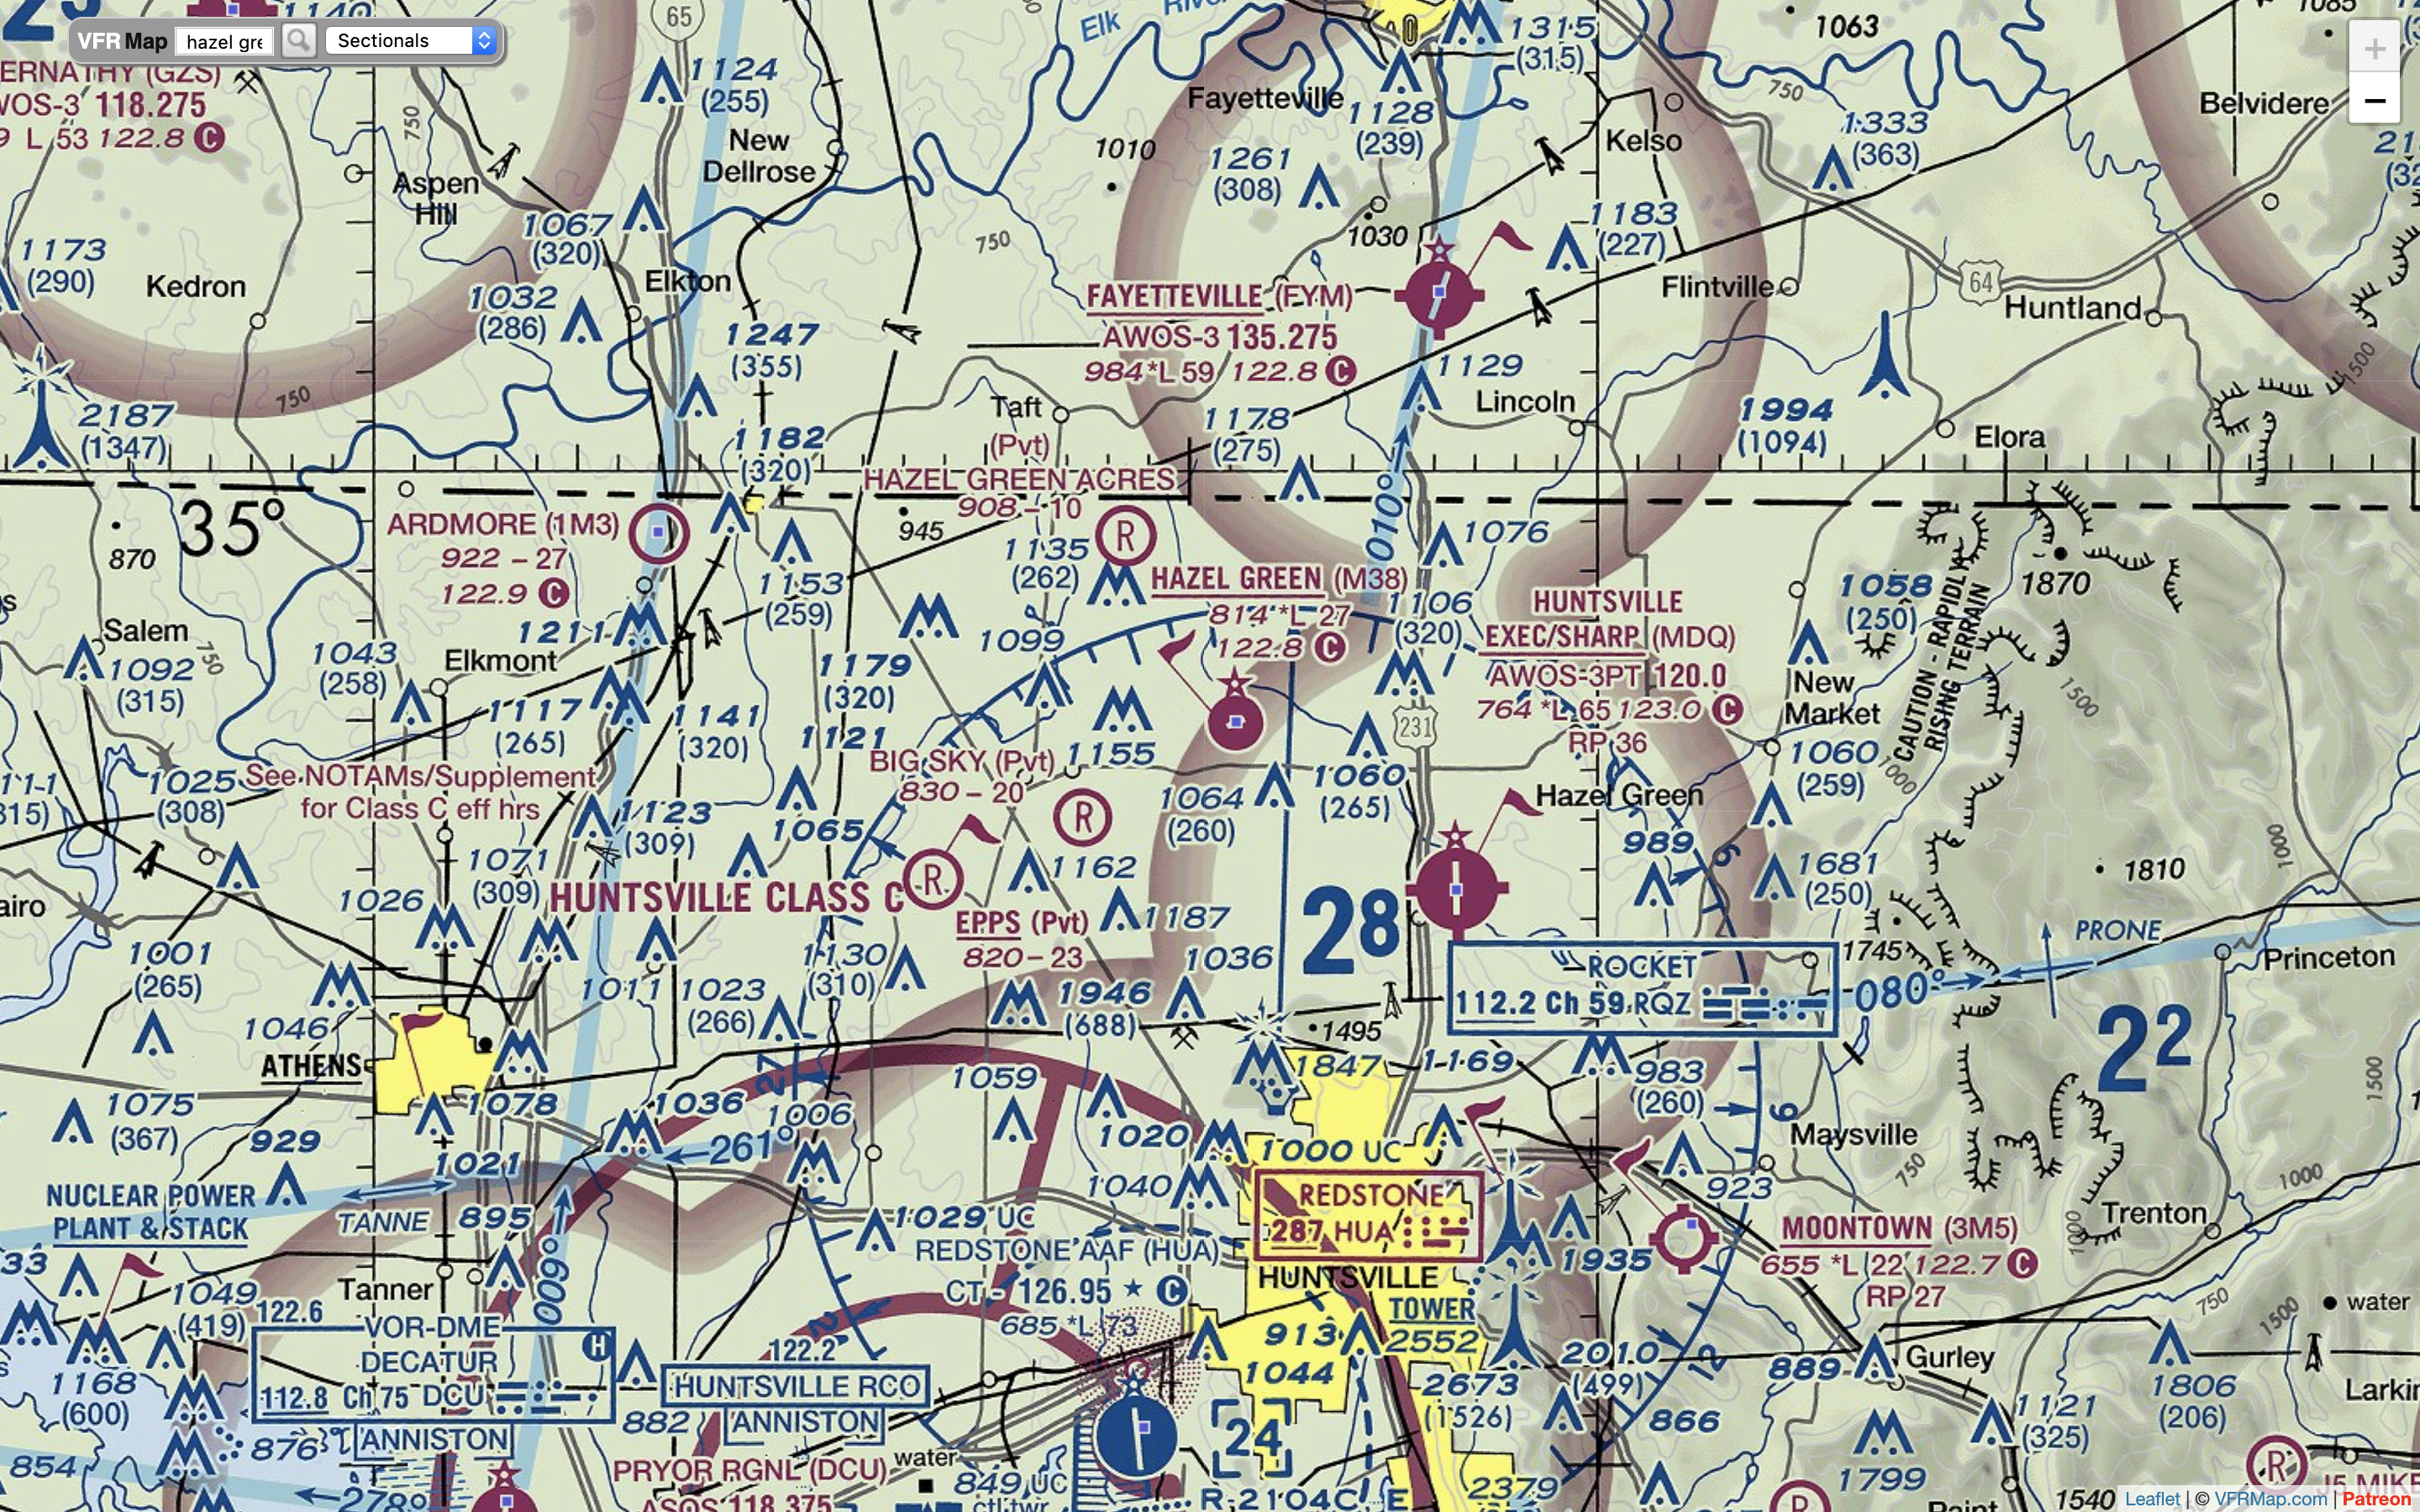
\includegraphics[width=0.75\linewidth]{img/PL/AeronauticalChart}
	\caption[VFR aeronautical chart of the Hazel Green, AL area]{\gls{vfr} aeronautical chart of the Hazel Green, AL area. Adapted from \href{http://vfrmap.com/}{VFRMap.com}}
	\label{fig:PL:Deployment:VFRchart}
\end{figure}

In this chart, the Class E airspace is bounded by a vignette magenta border, and spans down to \SI{700}{\feet}; anything below that is Class G airspace, and thus open for \gls{uav} operations. Incidentally, the area of payload operations lies beyond a 5 mile radius of the closest airfield.

\subsection{Team-derived requirements}

In addition to the above, a number of additional requirements have been compiled by the team. In particular, the robustness of the securement system, as well as the reliability of the deployment system are at the center of the discussion\todo[author=HE]{Draft team-derived requirements}.

\begin{enumerate}[noitemsep, label=\arabic*.]
	\item Deployment
	\begin{enumerate}[noitemsep, label=1.\arabic*.]
		\item UAV Transport 
		\begin{enumerate}[noitemsep, label=1.1.\arabic*.]
			\item The UAV must be securely transported from launch until deployment. There must be no physical damage to the UAV, and its functionality must be maintained.
			\item The security mechanism of the UAV and the UAV itself must be built to be able to withstand FILLER Gs. 
			\item This security mechanism must be released when the rocket reaches 120m as regulated by the FAA. 
		\end{enumerate}
		\item Nose Cone Release
		\begin{enumerate}[noitemsep, label=1.2.\arabic*.]
			\item The nose cone must be safely jettisoned to allow for proper UAV deployment. A safe jettison requires the nose cone's kinetic energy to be less than 100J as it impacts the ground.
			\item A parachute with an area of FILLER must deploy from its stored location in the tip of the nose cone in order to satisfy the kinetic energy requirement as shown in equation FILLER.
		\end{enumerate}
		\item UAV Release
		\begin{enumerate}[noitemsep, label=1.3.\arabic*.]
			\item The UAV must be safely lowered from the payload bay so that it can begin its independent flight.
			\item The lowering mechanism must be able to withstand a force greater than the weight of the UAV.
			\item The lowering mechanism must be able to deploy the UAV within ten seconds of the jettison of the nose cone.
		\end{enumerate}
		\item Critical Systems Check
		\begin{enumerate}[noitemsep, label=1.4.\arabic*.]
			\item A critical systems check must be performed quickly to ensure the UAV's ability to fly independently.
			\item The arms of the UAV must be properly deployed.
			\item The power system of the UAV must functional.
			\item The motors with propellers must be actively running.
			\item The orientation of the UAV must be upright as confirmed by accurate readings from the appropriate sensors.
		\end{enumerate}
		\item Separation Protocol
		\begin{enumerate}[noitemsep, label=1.5.\arabic*.]
			\item There must be a mechanism to detach the UAV from the upper body tube so that it can achieve independent flight.
			\item An automatic maneuver must be executed by the UAV to move itself away from the falling body tube.
		\end{enumerate}
	\end{enumerate}
	\item Hover
	\begin{enumerate}[noitemsep, label=2.\arabic*.]
		\item Take longer Kenneth
		\item \begin{enumerate}[noitemsep, label=2.1.\arabic*.]
			\item For real
		\end{enumerate}
	\end{enumerate}
	\item Landing Protocol
	\begin{enumerate}[noitemsep, label=3.\arabic*.]
		\item Computer Vision Check
		\begin{enumerate}[noitemsep, label=3.1.\arabic*.]
			\item The computer vision program must be working as designed as the UAV approaches GPS waypoint for the landing site of the sample material. The pilot will have to manually confirm that the system is functioning properly.
		\end{enumerate}
		\item IRMA System Check
		\begin{enumerate}[noitemsep, label=3.2.\arabic*.]
			\item The IRMA system must confirm its functionality post-deployment.
			\item The flight computer must confirm that the members of the IRMA can close to scoop the material. 
		\end{enumerate}
		\item UAV Descent on Target
		\begin{enumerate}[noitemsep, label=3.3.\arabic*.]
			\item The UAV must begin to descend towards the ground as it processes its final systems check.
			\item The descent velocity must be kept under FILLER m/s to ensure that any impact with a landing surface does not harm the UAV.
			\item The computer vision software must guide the UAV towards the sample collection site.
			\item The UAV must land upright atop the sample site with a final velocity of 0 m/s.
		\end{enumerate}
	\end{enumerate}
	\item Sample Retrieval Protocol
	\begin{enumerate}[noitemsep, label=4.\arabic*.]
		\item Engage IRMA
		\begin{enumerate}[noitemsep, label=4.1.\arabic*.]
			\item The IRMA must close its members around a collection of the sample.
			\item The UAV pilot must confirm that a sufficient that the IRMA has retrieved a sufficient amount of the sample.
		\end{enumerate}
		\item Return to Hover
		\begin{enumerate}[noitemsep, label=4.2.\arabic*.]
			\item The UAV must return to the altitude of the initial hover.
			\item The IRMA must maintain a sufficient amount of sample.
		\end{enumerate}
		\item Flee Sample Site
		\begin{enumerate}[noitemsep, label=4.3.\arabic*.]
			\item The UAV must move 5m in any cardinal direction from its location above the sample site.
		\end{enumerate}
	\end{enumerate}
\end{enumerate}

\section{Means of Securement}\label{PL:Deployment:Securement}
	\subsection{Locking Mechanism}
		This is a filler paragraph
		
	\subsection{UAV Arm Configuration}
		\subsubsection{Parallel Unfolding Arms}
			This is a filler paragraph

		\subsubsection{Vertically Unfolding Arms}
			This is a filler paragraph

\section{Means of Deployment}\label{PL:Deployment:Deployment}
	\subsection{UAV Release Mechanism}
		\subsubsection{Launch Rails}
			This is a filler paragraph

		\subsubsection{Lowering Mechanism}
			This is a filler paragraph

	\subsection{Nose Cone Jettison}
		\subsubsection{Without Parachute}
			This is a filler paragraph
		
		\subsubsection{With Parachute}
			This is a filler paragraph

\section{Payload Structures}\label{PL:Deployment:Structures}
	\subsection{Landing Leg Design}
		\subsubsection{Retractable Landing Mechanism}
			This is a filler paragraph

		\subsubsection{Static Landing Mechanism}
			This is a filler paragraph

	\subsection{Ice Retrieval and Mobility Agent}
		\subsubsection{Pin Joint Mechanism}
			This is a filler paragraph

		\subsubsection{Sliding Pin Mechanism}
			This is a filler paragraph

		\subsubsection{Wormgear Mechanism}
			This is a filler paragraph

\section{Payload Avionics}\label{PL:Deployment:Avionics}
	\subsection{Computer Vision}
		\subsubsection{Algorithmic Approach}
			This is a filler paragraph

		\subsubsection{Deep Learning Approach}
			This is a filler paragraph

	\subsection{Flight Controller}
		\subsubsection{ArduPilot}
			This is a filler paragraph

		\subsubsection{Pixhawk}
			This is a filler paragraph

		\subsubsection{Navio2}
			This is a filler paragraph

\section{Leading Design}\label{PL:Deployment:LeadingDesign}
	\subsection{Drone Structures}
		\subsubsection{Arm Configuration}
			This is a filler paragraph

		\subsubsection{Landing Legs}
			This is a filler paragraph
	
		\subsubsection{Ice Recovery and Mobility Agent}
			This is a filler paragraph

	\subsection{Avionics}
		\subsubsection{Flight Controller}
			This is a filler paragraph

		\subsubsection{Computer Vision}
			This is a filler paragraph

\section{Testing Campaign}\label{PL:Deployment:Testing}
	\subsection{Structual Testing}
		\subsubsection{Deployment Tests}
			This is a filler paragraph

		\subsubsection{Ice Retrieval and Mobility Agent Tests}
			This is a filler paragraph

	\subsection{Avionics Testings}
		\subsubsection{Flight Controller Tests}
			This is a filler paragraph

		\subsubsection{Computer Vision Tests}
			This is a filler paragraph







\chapter{Operational Protocols}

Throughout the mission, the \gls{uav} will encounter a number of varied tasks that must be completed sequentially so as to satisfy the mission objectives. As such, it is natural to define a number of regimes in which the vehicle must operate, as these dictate the operational protocols that are to be effectuated. This chapter details these operational regimes, including the pertinent operational protocols. Specifically, the following regimes are identified and discussed in due detail:

\begin{enumerate}[noitemsep, label=\Roman*.]
	\item Transit \& Deployment
	\item Descent
	\item Loiter
	\item Landing
	\item Retrieval
\end{enumerate}

\section{Transit \& Deployment}

Throughout stand-by, launch and passive descent, referred to as 'transit', the \gls{uav} will assume a low-power mode, periodically sending status updates and seeking connection with a ground station. This passive mode stems from multiple considerations. First, given the limited power supply, as much power as possible is to be saved will still maintaining a connection with the \gls{uav}. Second, by \gls{faa} regulations, the \gls{uav} may only be operated below \SI{400}{\feet} in \gls{los}\footnote{FAA Reauthorization Act of 2018 \S 346(b.2.C), 49 U.S.C. \S 44806} \citep{FederalAviationAdministration2018}. To ensure that no active operation takes place above this ceiling, the vehicle will restrict its operations by considering its current altimeter reading as a locking mechanism. This `altitude lock' constitutes the transit phase.

From the FAA Reauthorization Act of 2018, the following pertinent regulations may be found. The \gls{uav} must have a gross weight under \SI{4.4}{\poundm}, and must be operated:

\begin{enumerate}[noitemsep, label=(\roman*)]
	\item within or beyond visual \gls{los} of the operator;
	\item less than \SI{400}{\feet} above ground;
	\item during daylight conditions;
	\item within Class G airspace; and
	\item outside of 5 statute miles from any airport, heliport, seaplane base, spaceport, or other location with aviation activities.
\end{enumerate}

Regarding points (iv) and (v), it is found that the closest airport is the Hazel Green airport. However, the launch site, Bragg Farms, is located outside of the Class E airspace, thus respecting the Class G airspace requirement  

 Given the fact that the payload will only be deployed upon being granted permission from the \gls{rso}, it is of importance to achieve a timely response in the event of late notification. In addition, proper coordination with the avionics systems is of importance, as solenoid disengagement and winch lowering must be followed by \gls{uav} arm deployment in close succession\todo[author=HE]{Expand on deployment requirements (robustness, rapidity) and ground proximity considerations}. 
 
\section{Descent}
 
\todo[author=HE]{Expand on descent phase, including trade-offs between guidance algorithms ((N)MPC, GPC) and waypoint tracking vs. visual guidance at close proximity (CV).}

Given the limited time of flight the \gls{uav} is capable of achieving, it is of importance to conclude the descent phase in as small of a time frame as possible. 

\section{Loiter}

\todo[author=HE]{Expand on loiter phase, highlighting energy efficiency and data acquisition (feature detection and path planning) during idle phase. Also detail what safety features must be incorporated into this phase (geofencing, no-fly zones have to default back to loiter).}

\section{Landing}

\todo[author=HE]{Expand on final approach and landing phase, including close-quarters operations and the role of computer vision in detecting the landing site, as well as the accuracy and terminal touch down conditions (velocity, attitude). Explain touch-and-go maneuvers in case of failed landing attempt.} 

\section{Retrieval}

\todo[author=HE]{Expand on retrieval protocol, including claw operations and validation of claw contents. Explain the details on distancing and safe idle mode after retrieval, as well as shutdown/hibernation routines.}

 

\chapter{Quadrotor Dynamic Model}

\section{Coordinate Systems}

Let us consider the following four coordinate systems: \begin{enumerate*}[label=(\roman*), noitemsep]
	\item inertial,
	\item Earth-fixed,
	\item instantaneous topocentric, and
	\item body-fixed
\end{enumerate*} \citep[pp.~3\textit{f.}]{Singh1975}. For these systems, the axes are defined as follows:

\textit{Inertial system ($\text{O}$ at Earth center)}

\begin{itemize}[noitemsep]
	\item[\textbf{X}] On the Earth equatorial plane, pointing to the zero longitude at take-off
	\item[\textbf{Y}] On the Earth equatorial plane, pointing to the \SI{90}{\degree} longitude at take-off
	\item[\textbf{Z}] Perpendicular to the equatorial plane, pointing to the North Pole
\end{itemize}

\textit{Earth-fixed system ($\text{O}_\text{E}$ at Earth center)}

\begin{itemize}[noitemsep]
	\item[$\mathbf{X_E}$] On the Earth equatorial plane, always pointing to the Greenwich (\SI{0}{\degree}) longitude
	\item[$\mathbf{Y_E}$] On the Earth equatorial plane, always pointing to the \SI{90}{\degree} longitude
	\item[$\mathbf{Z_E}$] Perpendicular to the equatorial plane, pointing to the North Pole
\end{itemize}

\textit{Instantaneous topocentric system ($\text{O}_\text{T}$ at the projection point of the moving \gls{uav} on the Earth surface)}

\begin{itemize}[noitemsep]
	\item[$\mathbf{x_T}$] On the local horizon plane tangent to the instantaneous projection point of the \gls{uav}, directed along the local geocentric North
	\item[$\mathbf{y_T}$] On the local horizon plane tangent to the instantaneous projection point of the \gls{uav}, directed along the local geocentric North
	\item[$\mathbf{z_T}$] Perpendicular to the instantaneous tangent plane, directed along the geocentric radius vector and pointing toward the Earth center
\end{itemize}

\textit{Body-fixed system ($\text{O}_\text{B}$ at the center of gravity of the \gls{uav})}

\begin{itemize}[noitemsep]
	\item[$\mathbf{x_B}$] Along the \gls{uav} principle (longitudinal) axis, positive forward
	\item[$\mathbf{y_B}$] Normal to the $x_B$--$z_B$ symmetric plane, completing the right-hand system
	\item[$\mathbf{z_B}$] In the principle plane of symmetry of the \gls{uav}, perpendicular to the $x_B$ axis and positive downward
\end{itemize}

We will chiefly confine our discussion to the $O_T$ (instantaneous topocentric system) and $O_B$ (body-fixed) frames, as the distances the vehicle will travel allow for a flat Earth approximation with constant uniform gravity \citep{Burko2005}. Let us now consider the coordinate transformation between these two frames:

\subsection{Coordinate Transformation}

Let us define the following Euler angles:

\begin{itemize}[noitemsep]
	\item[$\boldsymbol{\theta}$] Pitch
	\item[$\boldsymbol{\psi}$] Yaw
	\item[$\boldsymbol{\phi}$] Roll
\end{itemize}

We then find the transformation from the instantaneous topocentric frame to the body-centric frame to be \citep[Eq.~2-2]{Kurak2018}:

\begin{equation}
\begin{split}
	[R]_{T \rightarrow B} (\theta, \psi, \phi) &=
	\begin{bmatrix}
		1 & 0 & 0 \\
		0 & \cos\phi & \sin\phi \\
		0 & -\sin\phi & \cos\phi
	\end{bmatrix}
	\begin{bmatrix}
		\cos\theta & 0 & -\sin\theta \\
		0 & 1 & 0 \\
		\sin\theta & 0 & \cos\theta
	\end{bmatrix}
	\begin{bmatrix}
		\cos\psi & \sin\psi & 0 \\
		-\sin\psi & \cos\psi & 0 \\
		0 & 0 & 1
	\end{bmatrix} \\
	&= 
	\begin{bmatrix}
		\cos\theta \cos\psi & \cos\theta \sin\psi & -\sin\theta \\
			\sin\theta \cos\psi \sin\phi - \sin\psi \cos\phi & \sin\theta \sin\psi \sin\phi + \cos\psi \cos\phi & \cos\theta \sin\phi \\
			\sin\theta \cos\psi \cos\phi + \sin\psi \sin\phi & \sin\theta \sin\psi \cos\phi - \cos\psi \sin\phi & \cos\theta \cos\phi \\
	\end{bmatrix}
\end{split}
\end{equation}

Given the nature of the transformation matrix, it is readily found that:

\begin{equation}
	[R]_{B \rightarrow T} = [R]_{T \rightarrow B}^{-1} = [R]_{T \rightarrow B}^\intercal
\end{equation}

\section{Dynamic Model}

Given the complex nature of the rotor-based \gls{uav}, we will make the following a priori assumptions to aid in the derivation of the vehicle model:

\begin{enumerate}[noitemsep]
	\item The \gls{uav} is a rigid body.
	\item The \gls{toi} of the \gls{uav} is approximated as the \gls{moi} of several objects.
	\item The \gls{cm} coincides with the \gls{uav}'s geometrical centroid.
	\item The \gls{moi} of the propellers is neglected.
	\item Time delay of commands is neglected.
	\item Aerodynamic drag force is neglected.
\end{enumerate}

While most of the aforestated simplifications are intuitively sound, neglecting the aerodynamic drag force begs for justification. \citet{Castillo2017} provide the following approximation to the \gls{uav} drag force:

\begin{equation}
	\vec{f}_{d_k} = C_{D_k} \rho A_k V_k (V_{w_k} - V_k) \hat{\vec{k}}, \quad k: x_b, y_b, z_b 
\end{equation} 

Where $\hat{\vec{k}}$ is the unit vector in $\vec{k}$ direction, $A_k$ is the reference area by which the drag coefficient $C_{D_k}$ is determined in the $\vec{k}$-direction. $V_k$ and $V_{w_k}$ are the vehicle velocity and wind velocity in $O_B$, respectively, and $\rho$ is the air density, which is assumed to be constant. In this formulation, $C_{D_k}$ is to be determined through simulation (\gls{cfd}) or experiment. However, this poses a significant difficulty: the \gls{uav} consists of many distinct components with orientation and speed dependent drag characteristics, making the definition of a constant $C_{D_k}$ inadvisable. As a matter of fact, \citet{Castillo2017} treat the drag force as an unknown disturbance that is to be counteracted by the control system, thus warranting the term to be dropped.

Let us define $\vec{T}$ and $\vec{H}$, the thrust force and hub torque for every motor--propeller system, respectively. Research shows that these forces scale with the square of the angular rate of the propellor \citep{Kurak2018, Castillo2017, Winslow2018, Bershadsky2016, Luukkonen2011}, i.e.:

\begin{align}
	T_i &= k_T \omega_i^2 \\
	H_i &= k_H \omega_i^2
\end{align}

where $i$ denotes the $i$'th propeller, and we assume the propellers to be identical, yielding constant $k_T, k_H$. These coefficients can be found experimentally. Following the Newton--Euler approach presented by \citet{Kurak2018}, we find for a symmetric four-propeller \gls{uav} layout:

\begin{align}
	\ddot\phi &= \frac{\ell (T_2 - T_4) - (I_z - I_y) \dot\theta \dot\psi}{I_x} \\
	\ddot\theta &= \frac{\ell (T_3 - T_1) - (I_x - I_z) \dot\phi \dot\psi}{I_y} \\
	\ddot\psi &= \frac{(H_1 + H_3) - (H_2 + H_4) - (I_y - I_x)\dot\phi \dot\theta}{I_z} \\
	\ddot x &= \frac{(\cos\phi \sin\theta \cos\psi + \sin\phi \sin\psi) \sum_{i=1}^{4} T_i}{m} \\
	\ddot y &= \frac{(\cos\phi \sin\theta \sin\psi - \sin\phi \cos\psi) \sum_{i=1}^{4} T_i}{m} \\
	\ddot z &= \frac{(\cos\phi \cos\theta) \sum_{i=1}^{4} T_i - m g}{m}
\end{align}

where $I_k = I_{kk}, k:x,y,z$ are the diagonal elements of the \gls{toi} $\vec{I}$, $\ell$ is the $L_2$-distance between the propeller and the origin of the $O_B$-frame ($\ell$ is constant to satisfy symmetry).

\subsection{Nonlinear state space model}

Let us define the following state variable:

\begin{equation}
	\begin{split}
		\vec{x} = 
		\begin{bmatrix}
			\phi \\
			\dot\phi \\
			\theta \\
			\dot\theta \\
			\psi \\
			\dot\psi \\
			z \\
			\dot z \\
			x \\
			\dot x \\
			y \\
			\dot y
		\end{bmatrix}
		=
		\begin{bmatrix}
			x_1 \\
			x_2 = \dot{x}_1 \\
			x_3 \\
			x_4 = \dot{x}_3 \\
			x_5 \\
			x_6 = \dot{x}_5 \\
			x_7 \\
			x_8 = \dot{x}_7 \\
			x_9 \\
			x_{10} = \dot{x}_9 \\
			x_{11} \\
			x_{12} = \dot{x}_{11} \\
		\end{bmatrix}
	\end{split}
\end{equation}

The force control input is then defined as:

\begin{equation}
	\vec{u}^* =
	\begin{bmatrix}
		\sum_{i=1}^{4} T_i \\
		T_2 - T_4 \\
		T_3 - T_1 \\
		(H_1 + H_3) - (H_2 + H_4)
	\end{bmatrix}
\end{equation}

Defining the angular rate control input as:

\begin{equation}
	\vec{u} = 
	\begin{bmatrix}
		\omega_1^2 \\ \omega_2^2 \\ \omega_3^2 \\ \omega_4^2 \\
	\end{bmatrix}
\end{equation}

Using this definition, we find the force control input $\vec{u}^*$ to be related to the angular rate control input $\vec{u}$ as follows:

\begin{equation}
	\vec{u}^* =
	\begin{bmatrix}
		k_T & k_T & k_T & k_T \\
		0 & k_T & 0 & - k_T \\
		- k_T & 0 & k_T & 0 \\
		k_H & - k_H & k_H & - k_H
	\end{bmatrix}
	\vec{u}
\end{equation}

Let us now define the following constants:

\begin{align}
	a_1 &= \frac{I_y - I_z}{I_x} && a_2 = \frac{I_z - I_x}{I_y} && a_3 = \frac{I_x - I_y}{I_z} \\
	b_1 &= \frac{\ell}{I_x} &&b_2 = \frac{\ell}{I_y} &&b_3 = \frac{\ell}{I_3}
\end{align}

and the following rotations:

\begin{equation}\label{eq:rotations}
\begin{split}
	r_t &= \cos\phi \cos\theta \\
	r_x &= \cos\phi \sin\theta \cos\psi + \sin\phi \sin\psi \\
	r_y &= \cos\phi \sin\theta \sin\psi - \sin\phi \cos\psi 
\end{split}
\end{equation}

The nonlinear state space formulation is then found to be:

\begin{equation}\label{eq:nonlinearss}
	\dot{\vec{x}} =
	\begin{bmatrix}
		x_2 \\
		x_4 x_6 a_1 + b_1 u^*_2 \\
		x_4 \\
		x_2 x_6 a_2 + b_2 u^*_3 \\
		x_6 \\
		x_2 x_4 a_3 + b_3 u^*_4 \\
		x_8 \\
		-g + r_t(x_1, x_3) u^*_1 / m \\
		x_{10} \\
		r_x(x_1, x_3, x_5) u^*_1 / m \\
		x_{12} \\
		r_y(x_1, x_3, x_5) u^*_1 / m 
	\end{bmatrix}
\end{equation}

\subsection{Linearized state space model}

Let us apply a small angle approximation on Eq.~\ref{eq:rotations}, giving:

\begin{equation}\label{eq:rotationsSAM}
\begin{split}
	r_t &\approx 1 \\
	r_x &\approx \theta \\
	r_y &\approx \theta\psi - \phi \approx -\phi
\end{split}
\end{equation}

To linearize Eq.~\ref{eq:nonlinearss}, we must find a suitable equilibrium point, where $\dot{\vec{x}} = \vec{0}$. This holds for:

\begin{equation}
\begin{split}
	\bar{\vec{x}} &= \begin{bmatrix}
		0 & 0 & 0 & 0 & 0 & 0 & \bar{x}_7 & 0 & \bar{x}_9 & 0 & \bar{x}_{11}
	\end{bmatrix}^\intercal \\
	\bar{\vec{u}}^* &= 
	\begin{bmatrix}
		mg & 0 & 0 & 0
	\end{bmatrix}^\intercal
\end{split}
\end{equation}

Linearizing Eq.~\ref{eq:nonlinearss} about $(\bar{\vec{x}}, \bar{\vec{u}}^*)$, we obtain:

\begin{equation}
\begin{split}
	\vec{A} &= \eval[1]{\pd{\dot{\vec{x}}(\vec{x},\vec{u}^*)}{\vec{x}}}_{(\bar{\vec{x}}, \bar{\vec{u}}^*)} \\
	\vec{B} &= \eval[1]{\pd{\dot{\vec{x}}(\vec{x},\vec{u}^*)}{{\vec{u}^*}}}_{(\bar{\vec{x}}, \bar{\vec{u}}^*)}
\end{split}
\end{equation}

which yields the following state space formulation:

\begin{equation} \label{eq:linearss}
\begin{split}
	\dot{\vec{x}} &=
	\underbrace{
	\begin{bmatrix}
		0 & 1 & 0 & 0 & 0 & 0 & 0 & 0 & 0 & 0 & 0 & 0 \\
		0 & 0 & 0 & 0 & 0 & 0 & 0 & 0 & 0 & 0 & 0 & 0 \\
		0 & 0 & 0 & 1 & 0 & 0 & 0 & 0 & 0 & 0 & 0 & 0 \\
		0 & 0 & 0 & 0 & 0 & 0 & 0 & 0 & 0 & 0 & 0 & 0 \\
		0 & 0 & 0 & 0 & 0 & 1 & 0 & 0 & 0 & 0 & 0 & 0 \\
		0 & 0 & 0 & 0 & 0 & 0 & 0 & 0 & 0 & 0 & 0 & 0 \\
		0 & 0 & 0 & 0 & 0 & 0 & 0 & 1 & 0 & 0 & 0 & 0 \\
		0 & 0 & 0 & 0 & 0 & 0 & 0 & 0 & 0 & 0 & 0 & 0 \\
		0 & 0 & 0 & 0 & 0 & 0 & 0 & 0 & 0 & 1 & 0 & 0 \\
		0 & g & 0 & 0 & 0 & 0 & 0 & 0 & 0 & 0 & 0 & 0 \\
		0 & 0 & 0 & 0 & 0 & 0 & 0 & 0 & 0 & 0 & 0 & 1 \\
		-g & 0 & 0 & 0 & 0 & 0 & 0 & 0 & 0 & 0 & 0 & 0
	\end{bmatrix}
	}_{\vec{A}}
	\vec{x}
	+
	\underbrace{
	\begin{bmatrix}
		0 & 0 & 0 & 0 \\
		0 & b_1 & 0 & 0 \\
		0 & 0 & 0 & 0 \\
		0 & 0 & b_2 & 0 \\
		0 & 0 & 0 & 0 \\
		0 & 0 & 0 & b_3 \\
		0 & 0 & 0 & 0 \\
		1/m & 0 & 0 & 0 \\
		0 & 0 & 0 & 0 \\
		0 & 0 & 0 & 0 \\
		0 & 0 & 0 & 0 \\
		0 & 0 & 0 & 0
	\end{bmatrix}
	}_{\vec{B}^*}
	\vec{u}^* \\
	&= \vec{A} \vec{x}
	+
	\underbrace{
	\begin{bmatrix}
		0 & 0 & 0 & 0 \\
		0 & b_1 k_T & 0 & -b_1 k_T \\
		0 & 0 & 0 & 0 \\
		-b_2 k_T & 0 & b_2 k_T & 0 \\
		0 & 0 & 0 & 0 \\
		b_3 k_H & -b_3 k_H & b_3 k_H & -b_3 k_H \\
		0 & 0 & 0 & 0 \\
		\frac{k_T}{m} & \frac{k_T}{m} & \frac{k_T}{m} & \frac{k_T}{m} \\
		0 & 0 & 0 & 0 \\
		0 & 0 & 0 & 0 \\
		0 & 0 & 0 & 0 \\
		0 & 0 & 0 & 0 \\
	\end{bmatrix}
	}_{\vec{B}}
	\vec{u}
\end{split}
\end{equation}

\subsection{Discretization}

\gls{zoh} discretization of Eq.~\ref{eq:linearss}, gives for constant sampling time $h$:

\begin{equation}
\begin{split}
	\vec{\Phi} &= e^{\vec{A} h} = 
	\begin{bmatrix}
		1 & h & 0 & 0 & 0 & 0 & 0 & 0 & 0 & 0 & 0 & 0 \\
		0 & 1 & 0 & 0 & 0 & 0 & 0 & 0 & 0 & 0 & 0 & 0 \\
		0 & 0 & 1 & h & 0 & 0 & 0 & 0 & 0 & 0 & 0 & 0 \\
		0 & 0 & 0 & 1 & 0 & 0 & 0 & 0 & 0 & 0 & 0 & 0 \\
		0 & 0 & 0 & 0 & 1 & h & 0 & 0 & 0 & 0 & 0 & 0 \\
		0 & 0 & 0 & 0 & 0 & 1 & 0 & 0 & 0 & 0 & 0 & 0 \\
		0 & 0 & 0 & 0 & 0 & 0 & 1 & h & 0 & 0 & 0 & 0 \\
		0 & 0 & 0 & 0 & 0 & 0 & 0 & 1 & 0 & 0 & 0 & 0 \\
		0 & \frac{g h^2}{2} & 0 & 0 & 0 & 0 & 0 & 0 & 1 & h & 0 & 0 \\
		0 & g h & 0 & 0 & 0 & 0 & 0 & 0 & 0 & 1 & 0 & 0 \\
		-\frac{g h^2}{2} & -\frac{g h^3}{6} & 0 & 0 & 0 & 0 & 0 & 0 & 0 & 0 & 1 & h \\
		-g h & -\frac{g h^2}{2} & 0 & 0 & 0 & 0 & 0 & 0 & 0 & 0 & 0 & 1 \\
	\end{bmatrix} \\
	\vec{\Gamma} &= \int_0^h e^{\vec{A} s} \dif s \cdot \vec{B} =
	\begin{bmatrix}
		0 & \frac{1}{2} b_1 h^2 k_T & 0 & -\frac{1}{2} b_1 h^2 k_T \\
		0 & b_1 h k_T & 0 & b_1 (-h) k_T \\
		-\frac{1}{2} b_2 h^2 k_T & 0 & \frac{1}{2} b_2 h^2 k_T & 0 \\
		b_2 (-h) k_T & 0 & b_2 h k_T & 0 \\
		\frac{1}{2} b_3 h^2 k_H & -\frac{1}{2} b_3 h^2 k_H & \frac{1}{2} b_3 h^2 k_H &
		-\frac{1}{2} b_3 h^2 k_H \\
		b_3 h k_H & b_3 (-h) k_H & b_3 h k_H & b_3 (-h) k_H \\
		\frac{h^2 k_T}{2 m} & \frac{h^2 k_T}{2 m} & \frac{h^2 k_T}{2 m} & \frac{h^2 k_T}{2 m} \\
		\frac{h k_T}{m} & \frac{h k_T}{m} & \frac{h k_T}{m} & \frac{h k_T}{m} \\
		0 & \frac{1}{6} b_1 g h^3 k_T & 0 & -\frac{1}{6} b_1 g h^3 k_T \\
		0 & \frac{1}{2} b_1 g h^2 k_T & 0 & -\frac{1}{2} b_1 g h^2 k_T \\
		0 & -\frac{1}{24} b_1 g h^4 k_T & 0 & \frac{1}{24} b_1 g h^4 k_T \\
		0 & -\frac{1}{6} b_1 g h^3 k_T & 0 & \frac{1}{6} b_1 g h^3 k_T \\
	\end{bmatrix}
\end{split}
\end{equation}

with the following state space system:

\begin{equation}
	\vec{x}(k+1) = \vec{\Phi} \vec{x}(k) + \vec{\Gamma}\vec{u}(k)
\end{equation}

\section{Simulation}

From \citet{Tayebi2004}, we adopt the following values for our simulation:

\begin{table}[H]
	\centering
	\caption[Simulation parameters]{Simulation parameters \cite{Tayebi2004}}
	\label{tab:tayebiparams}
	\begin{tabularx}{.4\linewidth}{l X}
		\toprule
		\textbf{Parameter} & \textbf{Value} \\
		\midrule
		$g$ & \SI{9.81}{\meter\per\second\squared} \\
		$m$ & \SI{0.468}{\kilo\gram} \\
		$\ell$ & \SI{0.225}{\meter} \\
		$k_T$ & \SI{2.980e-6}{(\radian\squared\per\second\squared)\per\newton} \\
		$k_H$ & \SI{1.140e-7}{(\radian\squared\per\second\squared)\per\newton\meter} \\
		$I_x$ & \SI{4.856e-3}{\kilo\gram\per\meter\squared} \\
		$I_y$ & \SI{4.856e-3}{\kilo\gram\per\meter\squared} \\
		$I_z$ & \SI{8.801e-3}{\kilo\gram\per\meter\squared} \\
		\bottomrule \\
	\end{tabularx}
\end{table}

Letting $h = \SI{1e-3}{\second}$, we obtain:

\begin{equation}
\begin{split}
	\vec{\Phi} &= 
	\begin{bmatrix}
		1 & 0.001 & 0 & 0 & 0 & 0 & 0 & 0 & 0 & 0 & 0 & 0 \\
		0 & 1 & 0 & 0 & 0 & 0 & 0 & 0 & 0 & 0 & 0 & 0 \\
		0 & 0 & 1 & 0.001 & 0 & 0 & 0 & 0 & 0 & 0 & 0 & 0 \\
		0 & 0 & 0 & 1 & 0 & 0 & 0 & 0 & 0 & 0 & 0 & 0 \\
		0 & 0 & 0 & 0 & 1 & 0.001 & 0 & 0 & 0 & 0 & 0 & 0 \\
		0 & 0 & 0 & 0 & 0 & 1 & 0 & 0 & 0 & 0 & 0 & 0 \\
		0 & 0 & 0 & 0 & 0 & 0 & 1 & 0.001 & 0 & 0 & 0 & 0 \\
		0 & 0 & 0 & 0 & 0 & 0 & 0 & 1 & 0 & 0 & 0 & 0 \\
		0 & 4.905\times10^{-6} & 0 & 0 & 0 & 0 & 0 & 0 & 1 & 0.001 & 0 & 0
		\\
		0 & 0.00981 & 0 & 0 & 0 & 0 & 0 & 0 & 0 & 1 & 0 & 0 \\
		-4.905\times10^{-6} & -1.635\times10^{-9} & 0
		& 0 & 0 & 0 & 0 & 0 & 0 & 0 & 1 & 0.001 \\
		-0.00981 & -4.905\times10^{-6} & 0 & 0 & 0 & 0 & 0 & 0 & 0 & 0 & 0
		& 1 \\
	\end{bmatrix} \\
	\vec{\Gamma} &= 
	\begin{bmatrix}
		1 & 0.001 & 0 & 0 & 0 & 0 & 0 & 0 & 0 & 0 & 0 & 0 \\
		0 & 1 & 0 & 0 & 0 & 0 & 0 & 0 & 0 & 0 & 0 & 0 \\
		0 & 0 & 1 & 0.001 & 0 & 0 & 0 & 0 & 0 & 0 & 0 & 0 \\
		0 & 0 & 0 & 1 & 0 & 0 & 0 & 0 & 0 & 0 & 0 & 0 \\
		0 & 0 & 0 & 0 & 1 & 0.001 & 0 & 0 & 0 & 0 & 0 & 0 \\
		0 & 0 & 0 & 0 & 0 & 1 & 0 & 0 & 0 & 0 & 0 & 0 \\
		0 & 0 & 0 & 0 & 0 & 0 & 1 & 0.001 & 0 & 0 & 0 & 0 \\
		0 & 0 & 0 & 0 & 0 & 0 & 0 & 1 & 0 & 0 & 0 & 0 \\
		0 & 4.905\times10^{-6} & 0 & 0 & 0 & 0 & 0 & 0 & 1 & 0.001 & 0 & 0
		\\
		0 & 0.00981 & 0 & 0 & 0 & 0 & 0 & 0 & 0 & 1 & 0 & 0 \\
		-4.905\times10^{-6} & -1.635\times10^{-9} & 0
		& 0 & 0 & 0 & 0 & 0 & 0 & 0 & 1 & 0.001 \\
		-0.00981 & -4.905\times10^{-6} & 0 & 0 & 0 & 0 & 0 & 0 & 0 & 0 & 0
		& 1 \\
	\end{bmatrix} 
\end{split}
\end{equation}

\section{Controller Design}

This section details the controller setup and design for the \gls{uav}. We concern ourself chiefly with the servo problem, with path generation being delegated to the guidance law. Given the nature of the problem, we are forced to employ the \gls{lqr} methodology to tune the gains for this \gls{mimo} system.
	
\subsection{\gls{lqr} Tuning}

Following the guidelines from \citep{Franklin2002}, we are to work with the following cost function:

\begin{equation}
	\mathcal{J} = \rho \vec{x}^\intercal \vec{H}_w^\intercal \overline{\vec{Q}}_1 \vec{H}_w \vec{x} + \vec{u}^\intercal \vec{Q}_2 \vec{u}
\end{equation}

where $\vec{Q}$ is a diagonal matrix containing elements that equal the inverse of the square of the maximum deviation of the states/inputs of interest. The value of $\rho$ is to be tuned by trial and error, considering the properties of the response.

\paragraph{State weighting matrix.} Since we wish to have full state control with minimal deviations on every state, we will pose $\vec{H}_w = \vec{I}_{12}$. Given this choice of $\vec{H}_w$, we find $\overline{\vec{Q}}_1 = \vec{Q}_1$. We find $\overline{\vec{Q}}_1$ to be of the form:

\begin{equation}
	\overline{\vec{Q}}_1 =
	\begin{bmatrix}
		\Delta x_1^{-2} & 0 & \cdots & 0 \\
		0 & \Delta x_2^{-2} & \ddots & \vdots \\
		\vdots & \ddots & \ddots & 0 \\
		0 & \cdots & 0 & \Delta x_{12}^{-2} 
	\end{bmatrix}
\end{equation}

where the entries are tabulated in Tab.~\ref{tab:maximum state deviation}. The rationale behind the magnitude of these bounds lies in the mission objective of the \gls{uav}; we wish to accomplish minute maneuvering and near-stationary hovering with closely matching attitude and small slew rate. As can be seen from the values, we place a greater importance on the vertical ($z$-axis) motion, such that the vehicle can accomplish accurate terrain following and close-quarters operations close to the surface.

\begin{table}[H]
	\centering
	\caption{Maximum state deviation values for use in the $\overline{\vec{Q}}_1$ matrix in the \gls{lqr} routine}
	\label{tab:maximum state deviation}
	\begin{tabularx}{.55\linewidth}{l l X}
		\toprule
		\textbf{State} & \textbf{Variable} & \textbf{Maximum state deviation} \\
		\midrule
		$\Delta x_1$ & $\phi$ & $\SI{2.5}{\degree} \approx \SI{4.36e-2}{\radian}$ \\
		$\Delta x_2$ & $\dot\phi$ & $\SI{1.25}{\degree\per\second} \approx \SI{2.18e-2}{\radian\per\second}$ \\
		$\Delta x_3$ & $\theta$ & $\SI{2.5}{\degree} \approx \SI{4.36e-2}{\radian}$ \\
		$\Delta x_4$ & $\dot\theta$ & $\SI{1.25}{\degree\per\second} \approx \SI{2.18e-2}{\radian\per\second}$ \\
		$\Delta x_5$ & $\psi$ & $\SI{5}{\degree} \approx \SI{8.73e-2}{\radian}$ \\
		$\Delta x_6$ & $\dot\psi$ & $\SI{2.5}{\degree\per\second} \approx \SI{4.36e-2}{\radian\per\second}$ \\
		$\Delta x_7$ & $z$ & $\SI{0.025}{\meter}$ \\
		$\Delta x_8$ & $\dot z$ & $\SI{0.0125}{\meter\per\second}$ \\
		$\Delta x_9$ & $x$ & $\SI{0.05}{\meter}$ \\
		$\Delta x_{10}$ & $\dot x$ & $\SI{0.025}{\meter\per\second}$ \\
		$\Delta x_{11}$ & $y$ & $\SI{0.05}{\meter}$ \\
		$\Delta x_{12}$ & $\dot y$ & $\SI{0.025}{\meter\per\second}$ \\
		\bottomrule
	\end{tabularx}
\end{table}

\paragraph{Control weighting matrix.} For the control input, we wish to minimize the use of excessive throttle. We can accomplish this by setting $\Delta u_i = 2^{-1/2} \omega^2_{\text{max}}$ for $i \in [1,4]$. This will translate to a maximum of $\pm 71\%$ throttle on each rotor, yielding a thrust cap at the \gls{rms} value of the maximum thrust, $T_{\text{cap}} = T_{\text{max}}/\sqrt{2}$, if we assume it to vary as a sinusoid. Similar to the state weighting matrix, the control weighting matrix will assume the form of:

\begin{equation}
	\begin{bmatrix}
		\Delta u_1^{-2} & 0 & \cdots & 0 \\
		0 & \Delta u_2^{-2} & \ddots & \vdots \\
		\vdots & \ddots & \ddots & 0 \\
		0 & \cdots & 0 & \Delta u_{4}^{-2} 
	\end{bmatrix}
\end{equation}

Summarizing, we obtain the following cost function:

\begin{equation}
	\mathcal{J} = \rho \vec{x}^\intercal \vec{Q} \vec{x} + \vec{u}^\intercal \vec{Q}_2 \vec{u}
\end{equation}

\part{Safety}

\chapter{Safety Plan Overview}

The safety of all team members is of the absolute highest priority for the Illinois Space Society Student Launch team. Should a situation arise in which a project-critical choice needs to be made, safety is considered before the success of the project. The safety officer this year is Zana Essmyer, who is overseeing a small team to conduct a thorough analysis of any hazards the team may encounter this year throughout the design, construction, assembly, and launches of the rocket and payload. Zana and the safety team are also implementing plans and procedures to minimize the risk of associated hazards.

This year, using a combination of in-person briefings, online classes and thorough documentation, the team is actively encouraging participation in the adherence to safety procedures. Safety training is required for any member that wishes to participate in construction sessions or attend a launch. By keeping lists of safety-trained members and having experienced members actively involved at every build session, the team can ensure that everyone working in lab spaces understands safety protocol for both day-to-day work and potential emergency situations. Forthcoming checklists will also be developed to ensure total safety during the off-pad, on-pad and post flight procedures.

\section{Emergency Preparedness}

Though the Illinois Space Society strives to maintain a safe working environment during all phases of the competition, the team also recognizes that accidents remain a possibility even with the strictest safety precautions in place. With this in mind, emergency preparedness forms another pillar of the team's safety plan. First aid kits are easily accessible in all of the team's main workspaces, and the safety officer has familiarized herself with their contents. The kits themselves are up-to-date and include wound dressings, antibiotic ointments, painkillers, and antihistamines. For any injuries requiring more than basic first aid, medical facilities are available both on and off the University of Illinois campus.

\section{Incident Reporting}

In the rare event that an accident requiring first aid occurs, the primary goal is always to care for and assist the injured team member. That said, once the incident has passed, the safety team's next priority is to actively prevent accident reoccurrence. Any incident is to be reported immediately to the safety officer, and from there it will be her responsibility to speak to those involved and determine the exact cause of the accident. Review of an incident will be considered complete once the safety officer has surveyed the scenario to her satisfaction and offered recommendations to the team leadership on how to prevent similar incidents in the future.

If an incident happens to occur, a series of actions will enact. The non-injured team member will assess the situation for any immediate dangers before contacting the Safety Officer, Technical Manager, and, if needed, emergency personnel. The Safety Officer will document the incident. The safety team will then take action to prevent further incidents.

\section{Equipment Training}

In order to provide team members with the experience necessary to operate a wide array of equipment and tooling, the safety team provides tutorial sessions on all machinery and tooling that may be used during the course of construction that is provided in the Nuclear Engineering Laboratory. To that end, the safety team has duplicated or adapted manufacturer-provided operating procedures for these tools and uploaded them to the team's shared drive for easy access. A collection of all training documents can be found in APPENDIX D: ISS Common Materials and Equipment Training with information included for the following devices:

\begin{itemize}[noitemsep]
    \item Full Spectrum Laser Professional Series CO2 48"$\times$36"  Cutter
    \item  Ultimaker 2 Extended 3D Printer
    \item Milwaukee Sawzall Reciprocating Saw
    \item DeWalt 18V Wireless Power Drill
    \item Dremel 8200-1/28 12-Volt Max Cordless Rotary Tool
    \item G5000 RocketPoxy
    \item Grizzly Model G7297 12" Disc Sander
    \item Water-Cooled Diamond Table Saw
    \item Grizzly H2936 Vacuum Sanding Table
    \item GMC 16" Scroll Saw
    \item JET 15" Bench Drill Press
    \item Soldering Station
    \item Miscellaneous Hand Tools (Screwdrivers, Hammer, Clamps, etc.)
\end{itemize}

In order to operate this machinery, a team member must attend tutorial sessions or receive training separately from a member of the safety team or team management. In providing and requiring these sessions, the team not only reduces the risk of mishaps due to misuse of equipment, but also ensures redundancy in knowledge of construction techniques. The Safety Officer will host tutorial sessions for ESPL machinery at the beginning of the semester for all members before access will be granted.

\section[NAR/TRA Procedures]{\gls{nar}/\gls{tra} Procedures}

The team will comply with the ``High Power Rocket Safety Code'' provided on the \gls{nar} website that has been effective since August 2012. The 13-step code and Minimum Distance Table on the website will be reviewed by the safety officer. All members on the team will be required to read the safety code online as it is a relatively short list of codes. The rules set forth by the \gls{nar} High Power Rocketry Code will always be respected and followed as they are set to ensure the safety of people and the environment. The safety officer, team manager, and sub-team managers will always make sure to comply with the safety code and ensure the rest of the team is properly complying. A copy of the \gls{nar} High Power Rocketry Code is included in this report as App.~\ref{App:Safety:NARCode}. Additionally, sections \todo[author=HE]{Add sec. on hazardous operations} and \todo[author=HE]{Add sec. on risk mitigation} elaborate on the hazardous operations and mitigation of risks. Hazardous materials and proper protocol is detailed under section\todo[author=HE]{Add sec. on hazardous materials}.

\paragraph{\gls{nar} Mentor.}

Mark Joseph will be the \gls{nar} mentor for the ISS Student Launch team for this year's competition. In addition to his longtime involvement in the high-power rocketry community, Mark has worked with the ISS team for several years now in the NASA Space Grant, Intercollegiate Rocket Engineering, and Student Launch Competitions.

\chapter{Risk Assessment Overview}

To better prepare for issues that inevitably arise during any project of large scale and to prioritize the team's time, the safety team has conducted a thorough risk analysis based on incident severity. The safety team analyzed risks to the project, the environment, and above all, the health of team members during the construction process. The team used \acrfullpl{rac} to evaluate the various hazards to both personnel and the project. Table~\ref{tab:level of risk and member requirements} introduces the risk matrix and the risk assessment codes that will be used to classify risks throughout the rest of the safety section. Risks are color-coded based on their severity, and  discusses the team's response to these various levels.  defines the levels of severity as it relates to personnel, project, and environmental health. Table 9 defines individual instance probability and probability of occurrence throughout the entire project timeline.

\begin{table}[H]
    \centering
    \caption{Level of risk and member requirements}
    \label{tab:level of risk and member requirements}
    \begin{tabularx}{0.8\linewidth}{X c c c c}
        \toprule
       \multirow{2}{*}{\textbf{Probability}} & \multicolumn{4}{c}{\textbf{Severity}} \\
       \cmidrule(l){2-5}
        & 1---Catastrophic & 2---Critical & 3---Marginal & 4---Negligible \\
       \midrule
       A---Frequent & \cellcolor{red!25} 1A & \cellcolor{red!25} 2A & \cellcolor{orange!25} 3A & \cellcolor{green!25} 4A \\
       B---Probable & \cellcolor{red!25} 1B & \cellcolor{red!25} 2B & \cellcolor{orange!25} 3B & \cellcolor{green!25} 4B \\
       C---Occasional & \cellcolor{red!25} 1C & \cellcolor{orange!25} 2C & \cellcolor{orange!25} 3C & 4C \\
       D---Remote & \cellcolor{orange!25} 1D & \cellcolor{orange!25} 2D & \cellcolor{green!25} 3D & 4D \\
       E---Improbable & \cellcolor{green!25} 1E & \cellcolor{green!25} 2E & \cellcolor{green!25} 3E & 4E \\
       \bottomrule
    \end{tabularx}
\end{table}

\part{Project Plan}

\chapter{Budget}

\section{Structures and Recovery}

\begin{table}[H]
	\centering
	\begin{tabularx}{\linewidth}{l | X X l l l l}
		\toprule
		\textbf{ID} & \textbf{Item} & \textbf{Purpose} & \textbf{Number} & \textbf{Unit Cost} & \textbf{Total Cost} & \textbf{Owned?} \\
		\midrule
		\texttt{SR.\IDnumber} & Epoxy and resin & Structural joints & N.A. & 70 USD & 70 USD & \xmark \\
		\midrule
		\texttt{SR.\IDnumber} & 60''$\times$4'' (L$\times$W) Blue Tube & Upper and lower airframe & 1 & 90 USD & 90 USD & \cmark \\
		\midrule
		\texttt{SR.\IDnumber} & 12''$\times$4'' (L$\times$D) Blue Tube coupler & Main rocket coupler bay & 1 & 45 USD & 45 USD & \xmark \\
		\midrule
		\texttt{SR.\IDnumber} & 9''$\times$6'' (L$\times$D) Fiberglass tube & Fairing tube & 1 & 60 USD & 60 USD & \xmark \\
		\bottomrule
	\end{tabularx}
\end{table}

\appendix
\appendixpage

\chapter[NAR High-Power Rocketry Safety Code]{\gls{nar} High-Power Rocketry Safety Code}\label{App:Safety:NARCode}

\begin{center}
\textbf{High Power Rocket Safety Code}
\end{center}\par

\begin{center}
\textbf{Effective August 2012}
\end{center}\par

\setlength{\parskip}{8.04pt}
\begin{enumerate}
	\item Certification. I will only fly high power rockets or possess high power rocket motors that are within the scope of my user certification and required licensing.\par

	\item Materials. I will use only lightweight materials such as paper, wood, rubber, plastic, fiberglass, or when necessary ductile metal, for the construction of my rocket.\par

	\item Motors. I will use only certified, commercially made rocket motors, and will not tamper with these motors or use them for any purposes except those recommended by the manufacturer. I will not allow smoking, open flames, nor heat sources within 25-ft. of these motors.\par

	\item Ignition System. I will launch my rockets with an electrical launch system, and with electrical motor igniters that are installed in the motor only after my rocket is at the launch pad or in a designated prepping area. My launch system will have a safety interlock that is in series with the launch switch that is not installed until my rocket is ready for launch, and will use a launch switch that returns to the ``off''  position when released. The function of onboard energetics and firing circuits will be inhibited except when my rocket is in the launching position.\par

	\item Misfires. If my rocket does not launch when I press the button of my electrical launch system, I will remove the launcher’s safety interlock or disconnect its battery, and will wait 60 seconds after the last launch attempt before allowing anyone to approach the rocket.\par

	\item Launch Safety. I will use a 5-second countdown before launch. I will ensure that a means is available to warn participants and spectators in the event of a problem. I will ensure that no person is closer to the launch pad than allowed by the accompanying Minimum Distance Table. When arming onboard energetics and firing circuits I will ensure that no person is at the pad except safety personnel and those required for arming and disarming operations. I will check the stability of my rocket before flight and will not fly it if it cannot be determined to be stable. When conducting a simultaneous launch of more than one high power rocket I will observe the additional requirements of NFPA 1127.\par

	\item Launcher. I will launch my rocket from a stable device that provides rigid guidance until the rocket has attained a speed that ensures a stable flight, and that is pointed to within 20 degrees of vertical. If the wind speed exceeds 5 miles per hour I will use a launcher length that permits the rocket to attain a safe velocity before separation from the launcher. I will use a blast deflector to prevent the motor’s exhaust from hitting the ground. I will ensure that dry grass is cleared around each launch pad in accordance with the accompanying Minimum Distance table, and will increase this distance by a factor of 1.5 and clear that area of all combustible material if the rocket motor being launched uses titanium sponge in the propellant.\par

	\item Size. My rocket will not contain any combination of motors that total more than 40,960 N-sec (9208 pound-seconds) of total impulse. My rocket will not weigh more at liftoff than one-third of the certified average thrust of the high power rocket motor(s) intended to be ignited at launch.\par

	\item Flight Safety. I will not launch my rocket at targets, into clouds, near airplanes, nor on trajectories that take it directly over the heads of spectators or beyond the boundaries of the launch site, and will not put any flammable or explosive payload in my rocket. I will not launch my rockets if wind speeds exceed 20 miles per hour. I will comply with Federal Aviation Administration airspace regulations when flying, and will ensure that my rocket will not exceed any applicable altitude limit in effect at that launch site.\par

	\item Launch Site. I will launch my rocket outdoors, in an open area where trees, power lines, occupied buildings, and persons not involved in the launch do not present a hazard, and that is at least as large on its smallest dimension as one-half of the maximum altitude to which rockets are allowed to be flown at that site or 1500-ft., whichever is greater, or 1000-ft. for rockets with a combined total impulse of less than 160 N-sec, a total liftoff weight of less than 1500 grams, and a maximum expected altitude of less than 610 meters (2000-ft.).\par

	\item Launcher Location. My launcher will be 1500-ft. from any occupied building or from any public highway on which traffic flow exceeds 10 vehicles per hour, not including traffic flow related to the launch. It will also be no closer than the appropriate Minimum Personnel Distance from the accompanying table from any boundary of the launch site.\par

	\item Recovery System. I will use a recovery system such as a parachute in my rocket so that all parts of my rocket return safely and undamaged and can be flown again, and I will use only flame-resistant or fireproof recovery system wadding in my rocket.\par

	\item Recovery Safety. I will not attempt to recover my rocket from power lines, tall trees, or other dangerous places, fly it under conditions where it is likely to recover in spectator areas or outside the launch site, nor attempt to catch it as it approaches the ground.
\end{enumerate}\par
\chapter[Federal Aviation Regulations 14 CFR 107]{Federal Aviation Regulations 14 CFR, Part 107, Small Unmanned Aircraft Regulations}

The \acrfull{faa} rules for small unmanned aircraft (referred to as `\acrfullpl{uas}') operations other than model aircraft---Part 107 of \gls{faa} regulations--cover a broad spectrum of commercial and government uses for \acrshortpl{uav} weighing less than 55 pounds. This chapter lists the highlights of the rule.

\paragraph{Operating Requirements.} 
When you are manipulating the controls of a drone, always avoid manned aircraft and never operate in a careless or reckless manner. You must keep your drone within sight. Alternatively, if you use \gls{fpv} or similar technology, you must have a visual observer always keep your aircraft within unaided sight (for example, no binoculars). Neither you nor a visual observer can be responsible for more than one unmanned aircraft operation at a time.

You can fly during daylight (30 minutes before official sunrise to 30 minutes after official sunset, local time) or in twilight with appropriate anti-collision lighting. Minimum weather visibility is three miles from your control station. The maximum allowable altitude is 400 feet above the ground, higher if your drone remains within 400 feet of a structure. Maximum speed is 100 mph (87 knots).

You currently cannot fly a small \gls{uas} over anyone not directly participating in the operation, not under a covered structure, or not inside a covered stationary vehicle.  No operations from a moving vehicle are allowed unless you are flying over a sparsely populated area.

You can carry an external load if it is securely attached and does not adversely affect the flight characteristics or controllability of the aircraft. You also may transport property for compensation or hire within state boundaries provided the drone, including its attached systems, payload and cargo, weighs less than 55 pounds total and you obey the other flight rules. (Some exceptions apply to Hawaii and the District of Columbia.)

You can request a waiver of most restrictions if you can show your operation will provide a level of safety at least equivalent to the restriction from which you want the waiver.

\paragraph{Registration.}
Anyone flying under Part 107 has to register each drone they intend to operate. If your drone weighs less than \SI{55}{\poundm}, you can use the automated registration system.

\paragraph{Pilot Certification.}
To operate the controls of a small \gls{uas} under Part 107, you need a remote pilot certificate with a small \gls{uas} rating, or be under the direct supervision of a person who holds such a certificate

You must be at least 16 years old to qualify for a remote pilot certificate, and you can obtain it in one of two ways.

You may pass an initial aeronautical knowledge test at an \gls{faa}-approved knowledge testing center.

If you already have a Part 61 pilot certificate, you must have completed a flight review in the previous 24 months and you must take a small \gls{uas} online training course provided by the \gls{faa}.

If you have a Part 61 certificate, you will immediately receive a temporary remote pilot certificate when you apply for a permanent certificate. Other applicants will obtain a temporary remote pilot certificate upon successful completion of \gls{tsa} security vetting. We anticipate we will be able to issue temporary certificates within 10 business days after receiving a completed application.

\paragraph{\gls{uas} Certification.}
You are responsible for ensuring a drone is safe before flying, but the \gls{faa} does not require small \gls{uas} to comply with current agency airworthiness standards or obtain aircraft certification. For example, you will have to perform a preflight inspection that includes checking the communications link between the control station and the \gls{uas}.

\paragraph{Other Requirements.}
If you are acting as pilot in command, you have to comply with several other provisions of the rule:

\setlength{\parskip}{5.04pt}
\begin{itemize}
	\item {\fontsize{10pt}{12.0pt}\selectfont \textcolor[HTML]{333333}{You must make your drone available to the FAA for inspection or testing on request, and you must provide any associated records required to be kept under the rule.}\par}\par

	\item {\fontsize{10pt}{12.0pt}\selectfont \textcolor[HTML]{333333}{You must report any operation that results in serious injury, loss of consciousness, or property damage of at least \$500 to the FAA within 10 days}\par}
\end{itemize}\par

\paragraph{Waivers and Airspace Authorizations.}
The \gls{faa} can issue waivers to certain requirements of Part 107 if an operator demonstrates they can fly safely under the waiver without endangering other aircraft or people and property on the ground or in the air. Operations in Class G airspace are allowed without air traffic control permission. Operations in Class B, C, D and E airspace need \gls{atc} approval.

In November 2017, the \gls{faa} deployed the Low Altitude Authorization and Notification Capability (LAANC – pronounced ``LANCE'' ) for drone operators at several air traffic facilities in an evaluation to see how well the prototype system functions and to address any issues that arise during testing. A beta test expansion of the system began on April 30, 2018 to deploy LAANC incrementally at nearly 300 air traffic facilities covering approximately 500 airports. The final deployment will begin on September 13.

The \gls{faa} expects LAANC will ultimately provide near real-time processing of airspace authorization requests for drone operators nationwide. The system is designed to automatically approve most requests to operate in specific areas of airspace below designated altitudes.


\chapter[Federal Aviation Regulations 14 CFR 101]{Federal Aviation Regulations 14 CFR, Subchapter F, Part 101, Subpart C -- Amateur Rockets}

\textbf{§ 101.21 Applicability.}\par

\textbf{(a)} This subpart applies to operating unmanned rockets. However, a person operating an unmanned rocket within a restricted area must comply with § 101.25(b)(7)(ii) and with any additional limitations imposed by the using or controlling agency.\par

\textbf{(b)} A person operating an unmanned rocket other than an amateur rocket as defined in § 1.1 of this chapter must comply with 14 CFR Chapter III.\par

\textbf{§ 101.22 Definitions.}\par


\vspace{\baselineskip}
The following definitions apply to this subpart:\par

\textbf{(a)\textit{ Class 1 - Model Rocket}} means an amateur rocket that:\par

\begin{adjustwidth}{0.5in}{0.0in}
\textbf{(1)} Uses no more than 125 grams (4.4 ounces) of propellant;\par

\end{adjustwidth}

\begin{adjustwidth}{0.5in}{0.0in}
\textbf{(2)} Uses a slow-burning propellant;\par

\end{adjustwidth}

\begin{adjustwidth}{0.5in}{0.0in}
\textbf{(3)} Is made of paper, wood, or breakable plastic;\par

\end{adjustwidth}

\begin{adjustwidth}{0.5in}{0.0in}
\textbf{(4)} Contains no substantial metal parts; and\par

\end{adjustwidth}

\begin{adjustwidth}{0.5in}{0.0in}
\textbf{(5)} Weighs no more than 1,500 grams (53 ounces), including the propellant.\par

\end{adjustwidth}

\textbf{(b)\textit{ Class 2 - High-Power Rocket}} means an amateur rocket other than a model rocket that is propelled by a motor or motors having a combined total impulse of 40,960 Newton-seconds (9,208 pound-seconds) or less.\par

\textbf{(c)\textit{ Class 3 - Advanced High-Power Rocket}} means an amateur rocket other than a model rocket or high-power rocket.\par

\textbf{§ 101.23 General operating limitations.}\par

\textbf{(a)} You must operate an amateur rocket in such a manner that it:\par

\begin{adjustwidth}{0.5in}{0.0in}
\textbf{(1)} Is launched on a suborbital trajectory;\par

\end{adjustwidth}

\begin{adjustwidth}{0.5in}{0.0in}
\textbf{(2)} When launched, must not cross into the territory of a foreign country unless an agreement is in place between the United States and the country of concern;\par

\end{adjustwidth}

\begin{adjustwidth}{0.5in}{0.0in}
\textbf{(3)} Is unmanned; and\par

\end{adjustwidth}

\begin{adjustwidth}{0.5in}{0.0in}
\textbf{(4)} Does not create a hazard to persons, property, or other aircraft.\par

\end{adjustwidth}

\textbf{(b)} The \gls{faa} may specify additional operating limitations necessary to ensure that air traffic is not adversely affected, and public safety is not jeopardized.\par

\textbf{§ 101.25 Operating limitations for Class 2-High Power Rockets and Class 3-Advanced High Power Rockets.}\par

When operating \textit{Class 2-High Power Rockets} or \textit{Class 3-Advanced High Power Rockets}, you must comply with the General Operating Limitations of § 101.23. In addition, you must not operate \textit{Class 2-High Power Rockets} or \textit{Class 3-Advanced High Power Rockets} -\par

\textbf{(a)} At any altitude where clouds or obscuring phenomena of more than five-tenths coverage prevails;\par

\textbf{(b)} At any altitude where the horizontal visibility is less than five miles;\par

\textbf{(c)} Into any cloud;\par

\textbf{(d)} Between sunset and sunrise without prior authorization from the \gls{faa};\par

\textbf{(e)} Within 9.26 kilometers (5 nautical miles) of any airport boundary without prior authorization from the \gls{faa};\par

\textbf{(f)} In controlled airspace without prior authorization from the \gls{faa};\par

\textbf{(g)} Unless you observe the greater of the following separation distances from any person or property that is not associated with the operations:\par

\begin{adjustwidth}{0.5in}{0.0in}
\textbf{(1)} Not less than one-quarter the maximum expected altitude;\par

\end{adjustwidth}

\begin{adjustwidth}{0.5in}{0.0in}
\textbf{(2)} 457 meters (1,500-ft.);\par

\end{adjustwidth}

\textbf{(h)} Unless a person at least eighteen years old is present, is charged with ensuring the safety of the operation, and has final approval authority for initiating high-power rocket flight; and\par

\textbf{(i)} Unless reasonable precautions are provided to report and control a fire caused by rocket activities.\par

\textbf{§ 101.27 \gls{atc} notification for all launches.}\par

No person may operate an unmanned rocket other than a Class 1 - Model Rocket unless that person gives the following information to the \gls{faa} \gls{atc} facility nearest to the place of intended operation no less than 24 hours before and no more than three days before beginning the operation:\par

\textbf{(a)} The name and address of the operator; except when there are multiple participants at a single event, the name and address of the person so designated as the event launch coordinator, whose duties include coordination of the required launch data estimates and coordinating the launch event;\par

\textbf{(b)} Date and time the activity will begin;\par

\textbf{(c)} Radius of the affected area on the ground in nautical miles;\par

\textbf{(d)} Location of the center of the affected area in latitude and longitude coordinates;\par

\textbf{(e)} Highest affected altitude;\par

\textbf{(f)} Duration of the activity;\par

\textbf{(g)} Any other pertinent information requested by the \gls{atc} facility.\par

\textbf{§ 101.29 Information requirements.}\par

\textbf{(a)\textit{ Class 2 - High-Power Rockets.}} When a \textit{Class 2 - High-Power Rocket} requires a certificate of waiver or authorization, the person planning the operation must provide the information below on each type of rocket to the \gls{faa} at least 45 days before the proposed operation. The \gls{faa} may request additional information if necessary to ensure the proposed operations can be safely conducted. The information shall include for each type of Class 2 rocket expected to be flown:\par

\begin{adjustwidth}{0.5in}{0.0in}
\textbf{(1)} Estimated number of rockets,\par

\end{adjustwidth}

\begin{adjustwidth}{0.5in}{0.0in}
\textbf{(2)} Type of propulsion (liquid or solid), fuel(s) and oxidizer(s),\par

\end{adjustwidth}

\begin{adjustwidth}{0.5in}{0.0in}
\textbf{(3)} Description of the launcher(s) planned to be used, including any airborne platform(s),\par

\end{adjustwidth}

\begin{adjustwidth}{0.5in}{0.0in}
\textbf{(4)} Description of recovery system,\par

\end{adjustwidth}

\begin{adjustwidth}{0.5in}{0.0in}
\textbf{(5)} Highest altitude, above ground level, expected to be reached,\par

\end{adjustwidth}

\begin{adjustwidth}{0.5in}{0.0in}
\textbf{(6)} Launch site latitude, longitude, and elevation, and\par

\end{adjustwidth}

\begin{adjustwidth}{0.5in}{0.0in}
\textbf{(7)} Any additional safety procedures that will be followed.\par

\end{adjustwidth}

\textbf{(b)\textit{ Class 3 - Advanced High-Power Rockets.}} When a \textit{Class 3 - Advanced High-Power Rocket} requires a certificate of waiver or authorization the person planning the operation must provide the information below for each type of rocket to the \gls{faa} at least 45 days before the proposed operation. The \gls{faa} may request additional information if necessary to ensure the proposed operations can be safely conducted. The information shall include for each type of Class 3 rocket expected to be flown:\par

\begin{adjustwidth}{0.5in}{0.0in}
\textbf{(1)} The information requirements of paragraph (a) of this section,\par

\end{adjustwidth}

\begin{adjustwidth}{0.5in}{0.0in}
\textbf{(2)} Maximum possible range,\par

\end{adjustwidth}

\begin{adjustwidth}{0.5in}{0.0in}
\textbf{(3)} The dynamic stability characteristics for the entire flight profile\par

\end{adjustwidth}

\begin{adjustwidth}{0.5in}{0.0in}
\textbf{(4)} A description of all major rocket systems, including structural, pneumatic, propellant, propulsion, ignition, electrical, avionics, recovery, wind-weighting, flight control, and tracking,\par

\end{adjustwidth}

\begin{adjustwidth}{0.5in}{0.0in}
\textbf{(5)} A description of other support equipment necessary for a safe operation,\par

\end{adjustwidth}

\begin{adjustwidth}{0.5in}{0.0in}
\textbf{(6)} The planned flight profile and sequence of events,\par

\end{adjustwidth}

\begin{adjustwidth}{0.5in}{0.0in}
\textbf{(7)} All nominal impact areas, including those for any spent motors and other discarded hardware, within three standard deviations of the mean impact point,\par

\end{adjustwidth}

\begin{adjustwidth}{0.5in}{0.0in}
\textbf{(8)} Launch commit criteria,\par

\end{adjustwidth}

\begin{adjustwidth}{0.5in}{0.0in}
\textbf{(9)} Countdown procedures, and\par

\end{adjustwidth}

\begin{adjustwidth}{0.5in}{0.0in}
\textbf{(10)} Mishap procedures.\par

\end{adjustwidth}

\bibliography{sources.bib}
	
\end{document}


